% !TEX encoding = UTF-8 Unicode

%----------------------------------------------------------------------------------------
%	PACKAGES AND OTHER DOCUMENT CONFIGURATIONS
%----------------------------------------------------------------------------------------

\documentclass[twoside]{article}

\usepackage[sc]{mathpazo} % Use the Palatino font
\usepackage[utf8]{inputenc}
\usepackage[english]{babel}
\usepackage[T1]{fontenc} % Use 8-bit encoding that has 256 glyphs
%\linespread{1.05} % Line spacing - Palatino needs more space between lines
\usepackage{microtype} % Slightly tweak font spacing for aesthetics

%\usepackage[hmarginratio=1:1,top=32mm,columnsep=20pt]{geometry} % Document margins
\usepackage[top=20mm,left=8mm,right=8mm,bottom=20mm]{geometry}

\usepackage{multicol} % Used for the two-column layout of the document
\usepackage[hang, small,labelfont=bf,up,textfont=it,up]{caption} % Custom capti
\usepackage{booktabs} % Horizontal rules in tables
\usepackage{float} % Required for tables and figures in the multi-column environment - they need to be placed in specific locations with the [H] (e.g. \begin{table}[H])
\usepackage{hyperref} % For hyperlinks in the PDF

\usepackage{lettrine} % The lettrine is the first enlarged letter at the beginning of the text
\usepackage{paralist} % Used for the compactitem environment which makes bullet points with less space between them

\usepackage{abstract} % Allows abstract customization
\renewcommand{\abstractnamefont}{\normalfont\bfseries} % Set the "Abstract" text to bold
\renewcommand{\abstracttextfont}{\normalfont\small\itshape} % Set the abstract itself to small italic text

%2º espacamento antes da section
\usepackage{titlesec} % Allows customization of titles
%\titlespacing*{\section}{0pt}{0pt}{0pt}
\renewcommand\thesection{\Roman{section}} % Roman numerals for the sections
\renewcommand\thesubsection{\Roman{subsection}} % Roman numerals for subsections
\titleformat{\section}[block]{\large\scshape\centering}{\thesection.}{1em}{} % Change the look of the section titles
\titleformat{\subsection}[block]{\large}{\thesubsection.}{1em}{} % Change the look of the section titles

\usepackage{fancyhdr} % Headers and footers
\pagestyle{fancy} % All pages have headers and footers
\fancyhead{} % Blank out the default header
\fancyfoot{} % Blank out the default footer
\fancyhead[C]{University of Minho $\bullet$ CPD Integrated Project 2015-2016} % Custom header text
\fancyfoot[RO,LE]{\thepage} % Custom footer text

%%% ADDED BY ME %%%%%%
%\floatstyle{boxed} 
\restylefloat{figure}
\usepackage{graphicx}
\usepackage{caption}
\usepackage{subcaption}
\usepackage{amsfonts}
\usepackage{listings,mdframed}
\usepackage{fancyvrb}
\usepackage{cleveref}
\usepackage{mathtools}
\usepackage{amsmath}
\usepackage{color}
\usepackage{relsize}
\usepackage{array}
\newcolumntype{L}[1]{>{\raggedright\let\newline\\\arraybackslash\hspace{0pt}}m{#1}}
\newcolumntype{C}[1]{>{\centering\let\newline\\\arraybackslash\hspace{0pt}}m{#1}}
\newcolumntype{R}[1]{>{\raggedleft\let\newline\\\arraybackslash\hspace{0pt}}m{#1}}
\usepackage{tabularx,caption}
\usepackage{multirow}

%%% For using norm || %%%%%
\newcommand{\norm}[1]{\left\lVert#1\right\rVert}

\newcommand*{\Package}[1]{\texttt{#1}}

\lstset{
    numbers=left,
	language=C,
	keywordstyle=\bfseries\ttfamily\color[rgb]{0,0,1},
	identifierstyle=\ttfamily,
	commentstyle=\color[rgb]{0.133,0.545,0.133},
	stringstyle=\ttfamily\color[rgb]{0.627,0.126,0.941},
	showstringspaces=false,
	basicstyle=\scriptsize,
numberstyle=\tiny,
numbers=right,
	stepnumber=1,
	numbersep=10pt,
	tabsize=1,
	breaklines=true,
	prebreak = \raisebox{0ex}[0ex][0ex]{\ensuremath{\hookleftarrow}},
	breakatwhitespace=false,
	aboveskip={1.5\baselineskip},
  columns=fixed,
  upquote=true,
  extendedchars=true,
 frame=single,
 inputencoding=utf8,
    literate={á}{{\'a}}1 {ã}{{\~a}}1 {â}{{\~a}}1 {é}{{\'e}}1 {ê}{{\'e}}1 {ç}{{\'c}}1 {ú}{{\'u}}1 {ó}{{\'o}}1 {í}{{\'i}}1,
 %backgroundcolor=\color{lbcolor},
}

\usepackage{blkarray}
\usepackage{stmaryrd}

%----------------------------------------------------------------------------------------
%	TITLE SECTION
%----------------------------------------------------------------------------------------

\title{\vspace{-15mm}\fontsize{24pt}{10pt}\selectfont\textbf{Optimisation of a Linear Algebra Approach to OLAP}} % Article title

\author{
\large
\textsc{Filipe Oliveira} - \textsc{A57816}\\
\normalsize \href{mailto:a57816@alunos.uminho.pt}{a57816@alunos.uminho.pt}
\vspace{-5mm}
\and
\textsc{Sérgio Caldas} - \textsc{A57779}\\
\normalsize \href{mailto:a57779@alunos.uminho.pt}{a57779@alunos.uminho.pt}
}



%----------------------------------------------------------------------------------------

\begin{document}

\maketitle % Insert title

\thispagestyle{fancy} % All pages have headers and footers

%----------------------------------------------------------------------------------------
%	ABSTRACT
%----------------------------------------------------------------------------------------

\begin{abstract}
\indent 
\par Online Analytical Processing (OLAP) systems, perform multidimensional analysis of business data and provides the capability for complex calculations, trend analysis, and sophisticated data modelling. 
Prior efforts have been made to prove that linear algebra (LA) is better suited than standard relational algebra(RA) for formalising and implementing queries in on-line multidimensional data analysis \cite{macedo2015linear} \cite{da2015benchmarking}, however, further work needed to be develop in order to specify and optimize parallel execution of the LA workflow.\par 
The proposed solution focus on a parallel typed linear algebra approach, enumerating how the Linear Algebra operations are efficiently implemented, giving preliminary experimental results obtained with one cluster of Search6 using queries of the TPC-H Benchmark, and comparing the achieved results with a parallel relational algebra engine -- PostgreSQL version 9.6. The first query of the TPC-H Benchmark was fully translated into LA operations to evaluate the performance of the Linear Algebra solution. As these experiments manage large amounts of data, two studies for sparse data representation were made in order to efficiently represent and access information in the LA approach.\par 
 By analysing the query results, we concluded that LA is extremely efficient in executing large data workflows, with benefits as datasets increase versus the RA approach.\par 
\end{abstract}
\vspace{0.5cm}

%----------------------------------------------------------------------------------------
%	ARTICLE CONTENTS
%----------------------------------------------------------------------------------------
\begin{multicols}{2} % Two-column layout throughout the main article text


% !TEX encoding = UTF-8 Unicode

\section{Introduction}
\indent

The design and development of systems that generate, collect, store, process, analyse, and query large sets of data is filled with significant challenges both hardware and software. Combined, these challenges represent a difficult landscape for software engineers.\par 
The relational database is the current solution for big data storage.
Data dependencies in databases can be seen as a binary two-way associative relation. 
Prior efforts have been made \cite{macedo2015linear} \cite{da2015benchmarking} towards a Linear Algebra (LA) approach to OLAP, in order to fully represent relational algebra in terms of linear algebra operators.
\par 

OLAP is resource-demanding and calls for efficient 	parallel approaches. 
We implemented from the start a typed linear algebra solution given special importance to the data modelling since it may limit the attainable efficiency in data-intensive systems such as OLAP, a time consuming task that accesses massive amounts. \par 
To validate the LA approach in a real case scenario and evaluate the outcome performance,the full set of TPC-H benchmarks was selected, with multiple query runs, and so far only one is reported in this work. To obtain realistic and meaningful results large datasets were considered, ranging from 1 to 32GB.\par 
For a comparative evaluation between the LA and the objected-relational database management system we selected PostgreSQL version 9.6, with roots in open source community,  to represent the relational algebra approach. \par 
Given this proximity between database relations and linear algebra, the question arises: does the linear algebra approach presents performance improvements when compared with the relational one?\par 

The following sections introduce the LA strategy (section \ref{strategy}), describe the experimental work with the sequential version of the code (section \ref{sequential}), introduce the parallelisation techniques to improve performance 	with experimental execution times \ref{parallel}, and the last section concludes with suggestions for later work.
\section{Linear Algebra Strategy}
\label{strategy}
\indent
\subsection{Towards a linear algebra semantics for SQL}

Inspired by point-free relational data processing, an alternative roadmap for parallel online analytical processing (OLAP) can be achieved based on encoding data in matrix format and relying thereupon solely on LA operations\cite{macedo2011middle}. 

\subsubsection{Encoding data in matrix format}

As example of raw data consider the displayed table \ref{table:example_table} where each row records the order key, quantity, return flag, line status and ship date from an given TPC-H benchmark lineitem table. In order to facilitate data association the column number in the corresponding lineitem table was included above each data column.
% !TEX encoding = UTF-8 Unicode

\begin{table}[H]


\caption{ Collection of raw data (adapted from TPC-H benchmark lineitem table). }
\label{table:example_table}
\scriptsize
\centering
\begin{tabular}{ |  L{1.5cm} |  L{1.5cm}  |  L{1.5cm}  |  L{1.5cm}  |  L{1.5cm} |   } 
\hline
\#1	&	\#5	&	\#9	&	\#10	&	\#11	  \\ 
l\_orderkey	&	l\_quantity	&	l\_returnflag	&	l\_linestatus	&	 l\_shipdate 	  \\ \hline
\hline
1	&	17	&	N	&	O	&	1996-03-13	  \\ \hline
1	&	36	&	N	&	O	&	1996-04-12	  \\ \hline
1	&	8	&	N	&	O	&	1996-01-29	  \\ \hline
1	&	28	&	N	&	O	&	1996-04-21	  \\ \hline
1	&	24	&	N	&	O	&	1996-03-30	  \\ \hline
1	&	32	&	N	&	O	&	1996-01-30	  \\ \hline
2	&	38	&	N	&	O	&	1997-01-28	  \\ \hline
3	&	45	&	R	&	F	&	1994-02-02	  \\ \hline
3	&	49	&	R	&	F	&	1993-11-09	  \\ \hline
3	&	27	&	A	&	F	&	1994-01-16	  \\ \hline
\end{tabular}
\end{table}


To obtain useful information from raw data, which in OLAP systems escalated to Terabytes of information, we need to summarise the data by selecting attributes of interest and exhibiting their inter-relationships.\par 
Consider the following simplified TPC-H query 1: "How many items were sold per return flag and line status?". For this particular question, the necessary attributes to answer the query are present on table lineitem, being \textbf{return flag}, \textbf{line status}, and \textbf{quantity}. In relational algebra that question could be easily expressed by the following SQL code, which would produce the result presented on table \ref{table:results_simple_query_1}.

\lstinputlisting[caption=SQL code for the simplified TPC-H query 1, label=simple_query_1]{sql/simple_query_1.sql} %input de um ficheiro


% !TEX encoding = UTF-8 Unicode
\begin{table}[H]
\caption{Simplified query-1 relational algebra result from the collection of raw data (adapted from TPC-H benchmark lineitem table). }
\label{table:results_simple_query_1}
\scriptsize
\centering
\begin{tabular}{ |  L{1.5cm} |  L{1.5cm}  |  L{1.5cm}  |    } 
\hline
\#9	&	\#10		 & \#5	  \\ 
l\_returnflag	&	l\_linestatus	&	 l\_quantity 	  \\ \hline
\hline
N	&	O	&	183	  \\ \hline
R	&	F	&	94	  \\ \hline
A	&	F	&	27	  \\ \hline
\end{tabular}

\end{table}


Aggregations like the ones presented on this query occur in all TPC-H queries, hence performance of group-by and aggregation deserves a special attention.
This issue will be addressed in later sections of the report.\par 
To express OLAP queries in therms of LA, the key lies in expressing operations in the form of matrix algebra expressions. 
This particular example, requires three matrices, one for each attribute, with each matrix being correlated to relational algebra as the row storage of columns \#5, \#9, and \#10.

However, to do so, we need to find a two-way association between the presented string on the rows \#9 and \#10 and an unique integer identifier. 

Our proposed solution encodes strings recurring to Gnome \textbf{Gquarks} - a two-way association between a non-zero unsigned int and a char * - based on a thread safe hashtable. \par 

By order of appearance, each unique string will be associated to an unique unsigned integer. Repeated strings will be associated to the prior corresponding unsigned integer. The resulting unsigned integer value range will start in the number 1. 

The value 0 in GQuarks is associated to NULL. 
Since in the proposed solution, row and column numbers will respect C-style arrays notation, both column and row numbering will start at 0. 

The GQuark unsigned integer value decremented by 1  will represent the row position on the matrix, and the register number, starting at 0, will represent the column position on the matrix. \par 
We can now verify that at most one non-zero cell can be found in each column of the matrix, to maintain the two-way association between a register and its corresponding string (the matrix is "functional"). There is also the possibility of direct associating an register number with a value, wether integer or floating point. The referred matrices will be diagonal matrices, in which the element value is directly associated with the register.\par 
Two types of matrices have now been presented:
\label{definition_matrices}
\begin{enumerate}
\item Projection matrices - which recur to Gnome Gquarks, in which the Gquark decremented by 1, represents the row position of the matrix, and the register number, starting at 0,  represents the column position on the matrix.
\item Measure matrices -  direct associating a register number with a value, wether integer or floating point,  where the element value is directly associated with the register number, and consequently the column and row position.
\end{enumerate}
 
We can now build the necessary matrices for the given examples, as shown in figures  \ref{fig:example_matrix_5} to \ref{fig:example_matrix_10}. The two-way association between char* and unsigned integer is also presented in table \ref{table:association_quarks_row}, to aid the example comprehension. 

% !TEX encoding = UTF-8 Unicode
\begin{table}[H]
\caption{Two-Way association between GQuarks and Row Number, for rows \#9 and \#10 presented in the collection of raw data (adapted from TPC-H benchmark lineitem table). }
\label{table:association_quarks_row}
\scriptsize
\centering
\begin{tabular}{ |  L{1.5cm} |  L{1.5cm}  |  L{1.5cm}  |    } 
\hline
String	&	GQuark	&	Row \#	  \\ \hline
\hline
N	&	1	&	0	  \\ \hline
R	&	2	&	1	  \\ \hline
A	&	3	&	2	  \\ \hline
O	&	4	&	3	  \\ \hline
F	&	5	&	4	  \\ \hline
\end{tabular}

\end{table}


  \begin{figure}[H]
    \centering
    \caption{Dense measure matrix produced from the collection of raw data (adapted from TPC-H benchmark lineitem table), from column \#5 (quantity column).}
\[
\begin{blockarray}{ccccccccccc}
	&	c0	&	c1	&	c2	&	c3	&	c4	&	c5	&	c6	&	c7	&	c8	&	c9	\\
\begin{block}{c(cccccccccc)}
r0	&	17	&	0	&	0	&	0	&	0	&	0	&	0	&	0	&	0	&	0	\\
r1	&	0	&	36	&	0	&	0	&	0	&	0	&	0	&	0	&	0	&	0	\\
r2	&	0	&	0	&	8	&	0	&	0	&	0	&	0	&	0	&	0	&	0	\\
r3	&	0	&	0	&	0	&	28	&	0	&	0	&	0	&	0	&	0	&	0	\\
r4	&	0	&	0	&	0	&	0	&	24	&	0	&	0	&	0	&	0	&	0	\\
r5	&	0	&	0	&	0	&	0	&	0	&	32	&	0	&	0	&	0	&	0	\\
r6	&	0	&	0	&	0	&	0	&	0	&	0	&	38	&	0	&	0	&	0	\\
r7	&	0	&	0	&	0	&	0	&	0	&	0	&	0	&	45	&	0	&	0	\\
r8	&	0	&	0	&	0	&	0	&	0	&	0	&	0	&	0	&	49	&	0	\\
r9	&	0	&	0	&	0	&	0	&	0	&	0	&	0	&	0	&	0	&	27	\\
\end{block}
\end{blockarray}
 \]
    \label{fig:example_matrix_5}
    \end{figure}
        
\begin{figure}[H]
\centering
\caption{Dense projection matrix produced from the collection of raw data (adapted from TPC-H benchmark lineitem table), from column \#9 (return flag column) with 2-way association achieved recurring to GQuarks.}
\[
\begin{blockarray}{ccccccccccc}
	&	c0	&	c1	&	c2	&	c3	&	c4	&	c5	&	c6	&	c7	&	c8	&	c9	\\
\begin{block}{c(cccccccccc)}
r0	&	1	&	1	&	1	&	1	&	1	&	1	&	1	&	0	&	0	&	0	\\
r1	&	0	&	0	&	0	&	0	&	0	&	0	&	0	&	1	&	1	&	0	\\
r2	&	0	&	0	&	0	&	0	&	0	&	0	&	0	&	0	&	0	&	1	\\
\end{block}
\end{blockarray}
\]
    \label{fig:example_matrix_9}
\end{figure}

\begin{figure}[H]
\centering
\caption{Dense projection matrix produced from the collection of raw data (adapted from TPC-H benchmark lineitem table), from column \#10 (line status column) with 2-way association achieved recurring to GQuarks.}
\[
\begin{blockarray}{ccccccccccc}
	&	c0	&	c1	&	c2	&	c3	&	c4	&	c5	&	c6	&	c7	&	c8	&	c9	\\
\begin{block}{c(cccccccccc)}
r0	&	0	&	0	&	0	&	0	&	0	&	0	&	0	&	0	&	0	&	0	\\
r1	&	0	&	0	&	0	&	0	&	0	&	0	&	0	&	0	&	0	&	0	\\
r2	&	0	&	0	&	0	&	0	&	0	&	0	&	0	&	0	&	0	&	0	\\
r3	&	1	&	1	&	1	&	1	&	1	&	1	&	1	&	0	&	0	&	0	\\
r4	&	0	&	0	&	0	&	0	&	0	&	0	&	0	&	1	&	1	&	1	\\
\end{block}
\end{blockarray}
\]
\label{fig:example_matrix_10}
\end{figure}
    
    \subsection{Projection Operation}

The projection statement of the example query is in listing \ref{simple_query_1_only_select}.

\lstinputlisting[caption=SQL code for the simplified TPC-H query 1 only for the SELECT and GROUP BY statements, label=simple_query_1_only_select]{sql/simple_query_1_only_select.sql} %input de um ficheiro

 The typical case to reproduce a SELECT and GROUP BY statement on a relational algebra approach would be to remove certain columns of the lineitem table. 
 In the LA approach the process consists of joining the projection matrices of the selected attributes. 
 The final LA result should hold all possible combinations
of the projected attributes and no duplicated tuples. That can be achieved by doing several Khatri-Rao products, one for each tuple of attributes present in the statement.\par 
The corresponding LA encoding of the SQL statement from listing \ref{simple_query_1_only_select} is given by the equation \ref{eq:khatri_1}, which would produce the matrix presented in figure \ref{fig:example_matrix_krao}.
 
\begin{equation}
\centering
Projection\ Matrix\ =\ ReturnFlag\ \otimes LineStatus
\label{eq:khatri_1}
\end{equation}


  
\begin{figure}[H]
\centering
\caption{Projection matrix produced from the Khatri-Rao product between return flag and line status columns from lineitem table, from columns \#9 and \#10.}
\[
\begin{blockarray}{ccccccccccc}
		& c	0	& c	1	& c	2	& c	3	& c	4	& c	5	& c	6	& c	7	& c	8	& c	9	\\
\begin{block}{c(cccccccccc)}
r	0	&	0	&	0	&	0	&	0	&	0	&	0	&	0	&	0	&	0	&	0	\\
r	1	&	0	&	0	&	0	&	0	&	0	&	0	&	0	&	0	&	0	&	0	\\
r	2	&	0	&	0	&	0	&	0	&	0	&	0	&	0	&	0	&	0	&	0	\\
r	3	&	1	&	1	&	1	&	1	&	1	&	1	&	1	&	0	&	0	&	0	\\
r	4	&	0	&	0	&	0	&	0	&	0	&	0	&	0	&	0	&	0	&	0	\\
r	5	&	0	&	0	&	0	&	0	&	0	&	0	&	0	&	0	&	0	&	0	\\
r	6	&	0	&	0	&	0	&	0	&	0	&	0	&	0	&	0	&	0	&	0	\\
r	7	&	0	&	0	&	0	&	0	&	0	&	0	&	0	&	0	&	0	&	0	\\
r	8	&	0	&	0	&	0	&	0	&	0	&	0	&	0	&	0	&	0	&	0	\\
r	9	&	0	&	0	&	0	&	0	&	0	&	0	&	0	&	1	&	1	&	0	\\
r	10	&	0	&	0	&	0	&	0	&	0	&	0	&	0	&	0	&	0	&	0	\\
r	11	&	0	&	0	&	0	&	0	&	0	&	0	&	0	&	0	&	0	&	0	\\
r	12	&	0	&	0	&	0	&	0	&	0	&	0	&	0	&	0	&	0	&	0	\\
r	13	&	0	&	0	&	0	&	0	&	0	&	0	&	0	&	0	&	0	&	0	\\
r	14	&	0	&	0	&	0	&	0	&	0	&	0	&	0	&	0	&	0	&	1	\\
\end{block}
\end{blockarray}
\]
\label{fig:example_matrix_krao}
\end{figure}

Given the matrices A with dimensions $(m\ \times\ n)$ and B with dimensions $(o\ \times\ p)$, the resulting projection matrix has dimensions $(q\ \times\ r)$, being $q\ =\ m =\ o$ and $r = m \times o$. The resulting matrix dimensions can also be expressed as $(\ (\ m\ \times\ o\ )\ \times\ n)$ as shown in figure \ref{fig:example_matrix_krao}.\par

To produce the desired tuples  holding all possible combinations, the association between row number and tuple has to be created. Given two original matrices A with dimensions $(m\ \times\ n)$ and B with dimensions $(o\ \times\ p)$, and one produced projection matrix C via the Khatri-Rao product, to re-obtain both strings that produce each tuple, for every row R$_{C}$ from the C matrix, the corresponding R$_{A}$ from matrix A, and R$_{B}$ from matrix B, are given by the expression: 


\begin{equation} \label{eq:eq1}
\begin{split}
R_A = R_C / o \\
 R_B\ =\  R_C  \mathbin{\%}  o
\end{split}
\end{equation}

We can now build the corresponding association between tuples and the rows of matrix C, as shown in table \ref{table:la_results_simple_query_1_repeated}. 




\begin{table}[H]
\caption{Association between the produced projection matrix from the Khatri-Rao product between return flag and line status columns from lineitem table, from columns \#9 and \#10, and the corresponding produced tuples for every row of matrix C.}
\label{table:la_results_simple_query_1_repeated}
\scriptsize
\centering
\begin{tabular}{ |   L{1.2cm} |  L{1.2cm} |  L{0.5cm}  |  L{0.5cm}  |   L{1cm} |  L{1cm}  |  L{1cm}  | } 
\hline
	Row C	&	Column C	&	$R_A$	&	$R_B$&	String A	&	String B	&	Tuple\\ \hline
r	3	&	0	&	0	&	3	&	N	&	O	&	(	N	,	O	)	\\  \hline
r	3	&	1	&	0	&	3	&	N	&	O	&	(	N	,	O	)	\\ \hline
r	3	&	2	&	0	&	3	&	N	&	O	&	(	N	,	O	)	\\ \hline
r	3	&	3	&	0	&	3	&	N	&	O	&	(	N	,	O	)	\\ \hline
r	3	&	4	&	0	&	3	&	N	&	O	&	(	N	,	O	)	\\ \hline
r	3	&	5	&	0	&	3	&	N	&	O	&	(	N	,	O	)	\\ \hline
r	3	&	6	&	0	&	3	&	N	&	O	&	(	N	,	O	)	\\ \hline
r	9	&	7	&	1	&	4	&	R	&	F	&	(	R	,	F	)	\\ \hline
r	9	&	8	&	1	&	4	&	R	&	F	&	(	R	,	F	)	\\ \hline
r	14	&	9	&	2	&	4	&	A	&	F	&	(	A	,	F	)	\\ \hline
\end{tabular}
\end{table}

\subsection{Aggregation Operation}

As you can state by observing table \ref{table:la_results_simple_query_1_repeated} the SELECT SQL statement was reproduced, however, the GROUP BY operation still needs to be applied. 

To represent the GROUP BY operation we need to define an operator, a row vector commonly know as bang\cite{macedo2015linear}. \par 

Given a matrix C with dimensions $(\ (\ m\ \times\ o\ )\ \times\ n\ )$, a correctly typed bang vector would have dimension n and be totally filled with the value 1. Figure \ref{fig:example_bang} illustrates the  bang vector to be multiplied by matrix C,  to group the elements located in the same row of matrix C.\par 

\begin{figure}[H]
\centering
\caption{Projection matrix produced from the Khatri-Rao product between return flag and line status columns from lineitem table, from columns \#9 and \#10.}
\[
\begin{blockarray}{cc}
		& c	0	\\
\begin{block}{c(c)}
r	0	&	1	\\
r	1	&	1	\\
r	2	&	1	\\
r	3	&	1	\\
r	4	&	1	\\
r	5	&	1	\\
r	6	&	1	\\
r	7	&	1	\\
r	8	&	1	\\
r	9	&	1	\\
\end{block}
\end{blockarray}
\]
\label{fig:example_bang}
\end{figure}

The grouped LA encoding of the SQL statement from listing \ref{simple_query_1_only_select} is given by the equation \ref{eq:khatri_2}, resulting in the projection vector presented in figure \ref{fig:example_krao_bang}:
 
\begin{equation}
\centering
Projection\ Vector\ =\ (\ ReturnFlag\ \otimes LineStatus\ ) \times bang
\label{eq:khatri_2}
\end{equation}





\begin{figure}[H]
\centering
\caption{Projection vector produced from the product between Khatri-Rao product shown on figure \ref{fig:example_matrix_krao} and bang row vector show on figure \ref{fig:example_krao_bang}.}
\[
\begin{blockarray}{cc}
		& c	0	\\
\begin{block}{c(c)}
r	0	&	0	\\
r	1	&	0	\\
r	2	&	0	\\
r	3	&	1	\\
r	4	&	0	\\
r	5	&	0	\\
r	6	&	0	\\
r	7	&	0	\\
r	8	&	0	\\
r	9	&	1	\\
r	10	&	0	\\
r	11	&	0	\\
r	12	&	0	\\
r	13	&	0	\\
r	14	&	1	\\
\end{block}
\end{blockarray}
\]
\label{fig:example_krao_bang}
\end{figure}

Considering the value 0 as the non existing relation between atributes, we can simplify the given projection vector and produce the association between return flag and line status columns from lineitem table, based on expression \ref{eq:eq1}, as shown in table \ref{table:la_results_simple_query_1}.


\begin{table}[H]
\caption{Association between the produced projection vector from the Khatri-Rao product between return flag and line status columns from lineitem table, from columns \#9 and \#10, and the corresponding tuples.}
\label{table:la_results_simple_query_1}
\scriptsize
\centering
\begin{tabular}{ |  L{1cm} |  L{0.5cm}  |  L{0.5cm}  |   L{1cm} |  L{1cm}  |  L{1cm}  | } 
\hline
Row C \#		&	$R_A$	&	$R_B$	&	String A	&	String B	&	Tuple		\\
\hline
r	3	&	0	&	3	&	N	&	O	&	(	N	,	O	)	\\ \hline
r	9	&	1	&	4	&	R	&	F	&	(	R	,	F	)	\\ \hline
r	14	&	2	&	4	&	A	&	F	&	(	A	,	F	)	\\ \hline
\end{tabular}
\end{table}

To produce the results show on listing \ref{simple_query_1}, using the linear algebra approach, we need to associate to every distinct tuple the corresponding quantity. Expression \ref{eq:khatri_3} adds the quantity measure matrix to the LA encoding. All measure matrices, shall therefore be represented between double square brackets,  to simplify differentiation from the projection matrix type.
 
\begin{equation}
\centering
( (\ ReturnFlag\ \otimes LineStatus\ ) \times\ \ \llbracket Quantity \rrbracket )\ \times\ bang
\label{eq:khatri_3}
\end{equation}

In addition to the  association between row number and tuple, with the values 1 and 0 representing the existence or non-existence of the attributes association respectively, we now have a value associated to each tuple. 
Figure \ref{fig:final_matrix_krao_qtt_bang} illustrates the resultant matrix of the dot product between the Khatri-Rao product between return flag and line status columns, and the quantity measure matrix, from the given lineitem example table.


\begin{figure}[H]
\centering
\caption{Resultant matrix of the dot product between the Khatri-Rao product between return flag and line status columns, and the quantity measure matrix, produced from the LA expression \ref{eq:khatri_3}.}
\[
\begin{blockarray}{ccccccccccc}
		& c	0	& c	1	& c	2	& c	3	& c	4	& c	5	& c	6	& c	7	& c	8	& c	9	\\
\begin{block}{c(cccccccccc)}
r	0	&	0	&	0	&	0	&	0	&	0	&	0	&	0	&	0	&	0	&	0	\\
r	1	&	0	&	0	&	0	&	0	&	0	&	0	&	0	&	0	&	0	&	0	\\
r	2	&	0	&	0	&	0	&	0	&	0	&	0	&	0	&	0	&	0	&	0	\\
r	3	&	17	&	36	&	8	&	28	&	24	&	32	&	38	&	0	&	0	&	0	\\
r	4	&	0	&	0	&	0	&	0	&	0	&	0	&	0	&	0	&	0	&	0	\\
r	5	&	0	&	0	&	0	&	0	&	0	&	0	&	0	&	0	&	0	&	0	\\
r	6	&	0	&	0	&	0	&	0	&	0	&	0	&	0	&	0	&	0	&	0	\\
r	7	&	0	&	0	&	0	&	0	&	0	&	0	&	0	&	0	&	0	&	0	\\
r	8	&	0	&	0	&	0	&	0	&	0	&	0	&	0	&	0	&	0	&	0	\\
r	9	&	0	&	0	&	0	&	0	&	0	&	0	&	0	&	45	&	49	&	0	\\
r	10	&	0	&	0	&	0	&	0	&	0	&	0	&	0	&	0	&	0	&	0	\\
r	11	&	0	&	0	&	0	&	0	&	0	&	0	&	0	&	0	&	0	&	0	\\
r	12	&	0	&	0	&	0	&	0	&	0	&	0	&	0	&	0	&	0	&	0	\\
r	13	&	0	&	0	&	0	&	0	&	0	&	0	&	0	&	0	&	0	&	0	\\
r	14	&	0	&	0	&	0	&	0	&	0	&	0	&	0	&	0	&	0	&	27	\\
\end{block}
\end{blockarray}
\]
\label{fig:final_matrix_krao_qtt_bang}
\end{figure}

The dot product between the resultant matrix defined in figure \ref{fig:final_matrix_krao_qtt_bang} and the row bang vector defined in figure \ref{fig:example_krao_bang} would produce the final row vector represented in figure \ref{fig:final_row_vector}.

\begin{figure}[H]
\centering
\caption{Final row vector produced from the product between Khatri-Rao product shown on figure \ref{fig:final_matrix_krao_qtt_bang} and bang row vector show on \ref{fig:example_krao_bang}.}
\[
\begin{blockarray}{cc}
		& c	0	\\
\begin{block}{c(c)}
r	0	&	0	\\
r	1	&	0	\\
r	2	&	0	\\
r	3	&	183	\\
r	4	&	0	\\
r	5	&	0	\\
r	6	&	0	\\
r	7	&	0	\\
r	8	&	0	\\
r	9	&	94	\\
r	10	&	0	\\
r	11	&	0	\\
r	12	&	0	\\
r	13	&	0	\\
r	14	&	27	\\
\end{block}
\end{blockarray}
\]
\label{fig:final_row_vector}
\end{figure}

We have now defined the necessary operations to reproduce through linear algebra the relational algebra results shown in table \ref{table:results_simple_query_1}. Table \ref{table:la_results_simple_query_1_qtt} associates the generated tuples via the Khatri-Rao operation shown in figure \ref{fig:final_matrix_krao_qtt_bang} and the row vector bang as shown in expression \ref{eq:khatri_3}.

\begin{table}[H]
\caption{Association between the generated tuples via the Khatri-Rao operation shown on figure \ref{fig:final_matrix_krao_qtt_bang} and the row vector bang as shown on expression \ref{eq:khatri_3}.}
\label{table:la_results_simple_query_1_qtt}
\scriptsize
\centering
\begin{tabular}{ |  L{1cm} |  L{0.5cm}  |  L{0.5cm}  |   L{1cm} |  L{1cm}  |  L{1cm}  |    L{1cm}  | } 
\hline
Row C \#		&	$R_A$	&	$R_B$	&	String A	&	String B	&	Tuple	& Value	\\
\hline
r	3	&	0	&	3	&	N	&	O	&	(	N	,	O	) &	183 \\ \hline
r	9	&	1	&	4	&	R	&	F	&	(	R	,	F	) &	94 \\ \hline
r	14	&	2	&	4	&	A	&	F	&	(	A	,	F	) &	27 \\ \hline
\end{tabular}
\end{table}

\subsection{Selection Operation}
Given the obtained results, there is still one linear operation required to fully answer to a new query,  closer to the TPC-H query 1: "How many items were sold per return flag and line status, between the dates 
1996-04-12 and 1997-01-28?". For this particular question, the necessary attributes to answer the query remain present on the table lineitem, being the prior analysed \textbf{return flag}, \textbf{line status}, and \textbf{quantity}, with the addition of the selection attribute -- \textbf{shipdate}. In relational algebra that question could be easily expressed with the extension of the prior SQL code presented on listing \ref{simple_query_1}, which would produce the result presented on table \ref{table:results_query_1}:

\lstinputlisting[caption=SQL code for the simplified TPC-H query 1, label=query_1]{sql/tpch_query_1.sql} %input de um ficheiro


% !TEX encoding = UTF-8 Unicode
\begin{table}[H]
\caption{Query-1 relational algebra result from the collection of raw data (adapted from TPC-H benchmark lineitem table). }
\label{table:results_query_1}
\scriptsize
\centering
\begin{tabular}{ |  L{1.5cm} |  L{1.5cm}  |  L{1.5cm}  |    } 
\hline
\#9	&	\#10		 & \#5	  \\ 
l\_returnflag	&	l\_linestatus	&	 l\_quantity 	  \\ \hline
\hline
N	&	O	&	102	  \\ \hline
\end{tabular}
\end{table}


The same result could be computed on linear algebra operations by strictly restricting the values present on the matrix shown in figure \ref{fig:final_matrix_krao_qtt_bang}. 

By producing a measure selection matrix initially with its diagonal cells filled with  value 1, and by re-obtaining the string based on the corresponding GQuark of the selection column, comparing it with both keys ( \textbf{1996-04-12} and \textbf{1997-01-28} ), we can simply replace with value 0 all cells of the measure selection matrix that do not pass in the restriction.\par 
 On subsection \ref{matrix_format} the non validation of the comparison would result in the elimination of the element from the sparse representation, as we shall address later. 
 
 To simplify the visualisation process of the algorithm, this method will be used in this section.\par 
Expression \ref{eq:tpch_1} adds the selection measure matrix to the LA encoding. We now have projection, selection, and aggregation operations defined only in terms of linear algebra.
\begin{equation}
\centering
\scriptsize
( ( (\ ReturnFlag\ \otimes LineStatus\ ) \times\ \llbracket Selection \rrbracket\ )\ \times\ \llbracket Quantity \rrbracket )\ \times\ bang
\label{eq:tpch_1}
\end{equation}

Figure \ref{fig:example_restriction} illustrates the resultant measure selection matrix of the restriction of shipdate column, from the given lineitem example table. To assist its visualisation, table \ref{table:la_selection} associates the row value of shipdate for every register with the result of the selection process.


\begin{table}[H]
\caption{Association between row value of shipdate for every register with the result of the selection process, for a restriction of values between \textbf{1996-04-12} and \textbf{1997-01-28}.}
\label{table:la_selection}
\scriptsize
\centering
\begin{tabular}{ |  L{1cm} |  L{2cm}  |  L{1cm}  | } 
\hline
Row \#		&	 l\_shipdate 	&	Value	  \\ \hline	
		\hline

r	0	&	1996-03-13	&	FALSE	  \\ \hline	
r	1	&	1996-04-12	&	\textbf{TRUE}	  \\ \hline	
r	2	&	1996-01-29	&	FALSE	  \\ \hline	
r	3	&	1996-04-21	&	\textbf{TRUE}	  \\ \hline	
r	4	&	1996-03-30	&	FALSE	  \\ \hline	
r	5	&	1996-01-30	&	FALSE	  \\ \hline	
r	6	&	1997-01-28	&	\textbf{TRUE}	  \\ \hline	
r	7	&	1994-02-02	&	FALSE	  \\ \hline	
r	8	&	1993-11-09	&	FALSE	  \\ \hline	
r	9	&	1994-01-16	&	FALSE	  \\ \hline	
\end{tabular}
\end{table}

 \begin{figure}[H]
\centering
\caption{Measure selection matrix produced from the restriction of shipdate column to values between  \textbf{1996-04-12} and \textbf{1997-01-28}, from the given lineitem example table, from column \#11.}
\[
\begin{blockarray}{ccccccccccc}
		& c	0	& c	1	& c	2	& c	3	& c	4	& c	5	& c	6	& c	7	& c	8	& c	9	\\
\begin{block}{c(cccccccccc)}
r	0	&	0	&	0	&	0	&	0	&	0	&	0	&	0	&	0	&	0	&	0	\\
r	1	&	0	&	1	&	0	&	0	&	0	&	0	&	0	&	0	&	0	&	0	\\
r	2	&	0	&	0	&	0	&	0	&	0	&	0	&	0	&	0	&	0	&	0	\\
r	3	&	0	&	0	&	0	&	1	&	0	&	0	&	0	&	0	&	0	&	0	\\
r	4	&	0	&	0	&	0	&	0	&	0	&	0	&	0	&	0	&	0	&	0	\\
r	5	&	0	&	0	&	0	&	0	&	0	&	0	&	0	&	0	&	0	&	0	\\
r	6	&	0	&	0	&	0	&	0	&	0	&	0	&	1	&	0	&	0	&	0	\\
r	7	&	0	&	0	&	0	&	0	&	0	&	0	&	0	&	0	&	0	&	0	\\
r	8	&	0	&	0	&	0	&	0	&	0	&	0	&	0	&	0	&	0	&	0	\\
r	9	&	0	&	0	&	0	&	0	&	0	&	0	&	0	&	0	&	0	&	0	\\
\end{block}
\end{blockarray}
\]
\label{fig:example_restriction}
\end{figure}

Note that the selection process could occur both in the projection or the aggregation process with the restriction to be realised before the  bang operation. 

To otimize the operations, the selection should be performed in the initial stages of the query, since it reduces the amount of computation required later.\par 
 
To visualize the LA operations presented in expression \ref{eq:tpch_1}, the product between Khatri-Rao product was shown in figure \ref{fig:final_matrix_krao_qtt_bang}, the measure selection matrix was defined in figure \ref{fig:example_restriction}, the measure quantity matrix was defined in figure \ref{fig:example_matrix_5}, and the row bang vector was defined in figure \ref{fig:example_krao_bang}, these led to the final row vector presented on figure \ref{fig:final_row_vector_selection}.

\begin{figure}[H]
\centering
\caption{Final row vector produced from the product between Khatri-Rao product shown on figure \ref{fig:final_matrix_krao_qtt_bang}, the measure selection matrix define in figure \ref{fig:example_restriction}, the measure quantity matrix define in figure \ref{fig:example_matrix_5}, and the row bang vector defined in figure \ref{fig:example_krao_bang}.}
\[
\begin{blockarray}{cc}
		& c	0	\\
\begin{block}{c(c)}
r	0	&	0	\\
r	1	&	0	\\
r	2	&	0	\\
r	3	&	102	\\
r	4	&	0	\\
r	5	&	0	\\
r	6	&	0	\\
r	7	&	0	\\
r	8	&	0	\\
r	9	&	0	\\
r	10	&	0	\\
r	11	&	0	\\
r	12	&	0	\\
r	13	&	0	\\
r	14	&	0	\\
\end{block}
\end{blockarray}
\]
\label{fig:final_row_vector_selection}
\end{figure}

We have now defined the necessary operations to reproduce through linear algebra the relational algebra results shown on table \ref{table:results_query_1}. Table \ref{table:la_results_query_1} associates the generated  selected tuples via expression \ref{eq:tpch_1}.


\begin{table}[H]
\caption{Association between the generated  selected tuples via expression \ref{eq:tpch_1}.}
\label{table:la_results_query_1}
\scriptsize
\centering
\begin{tabular}{ |  L{1cm} |  L{0.5cm}  |  L{0.5cm}  |   L{1cm} |  L{1cm}  |  L{1cm}  |    L{1cm}  | } 
\hline
Row C \#		&	$R_A$	&	$R_B$	&	String A	&	String B	&	Tuple	& Value	\\
\hline
r	3	&	0	&	3	&	N	&	O	&	(	N	,	O	) &	102 \\ \hline
\end{tabular}
\end{table}

 

\subsection{Encoding data in Sparse Matrix Format}
\label{matrix_format}
The matrices used to encode OLAP information displau a high degree of both sparsity and irregularity. Regarding the minor dataset used in the experimental work, figures \ref{fig:sparse_1_5} trough \ref{fig:sparse_1_11}, analyse the sparsity pattern of the necessary columns, to answer the simplified TPC-H query-1 show on expression \ref{eq:tpch_1}.


\begin{figure}[H]
\centering
\caption{Sparsity pattern analysis for attribute quantity, from the TPC-H dataset 1GB lineitem table(column \#5).}
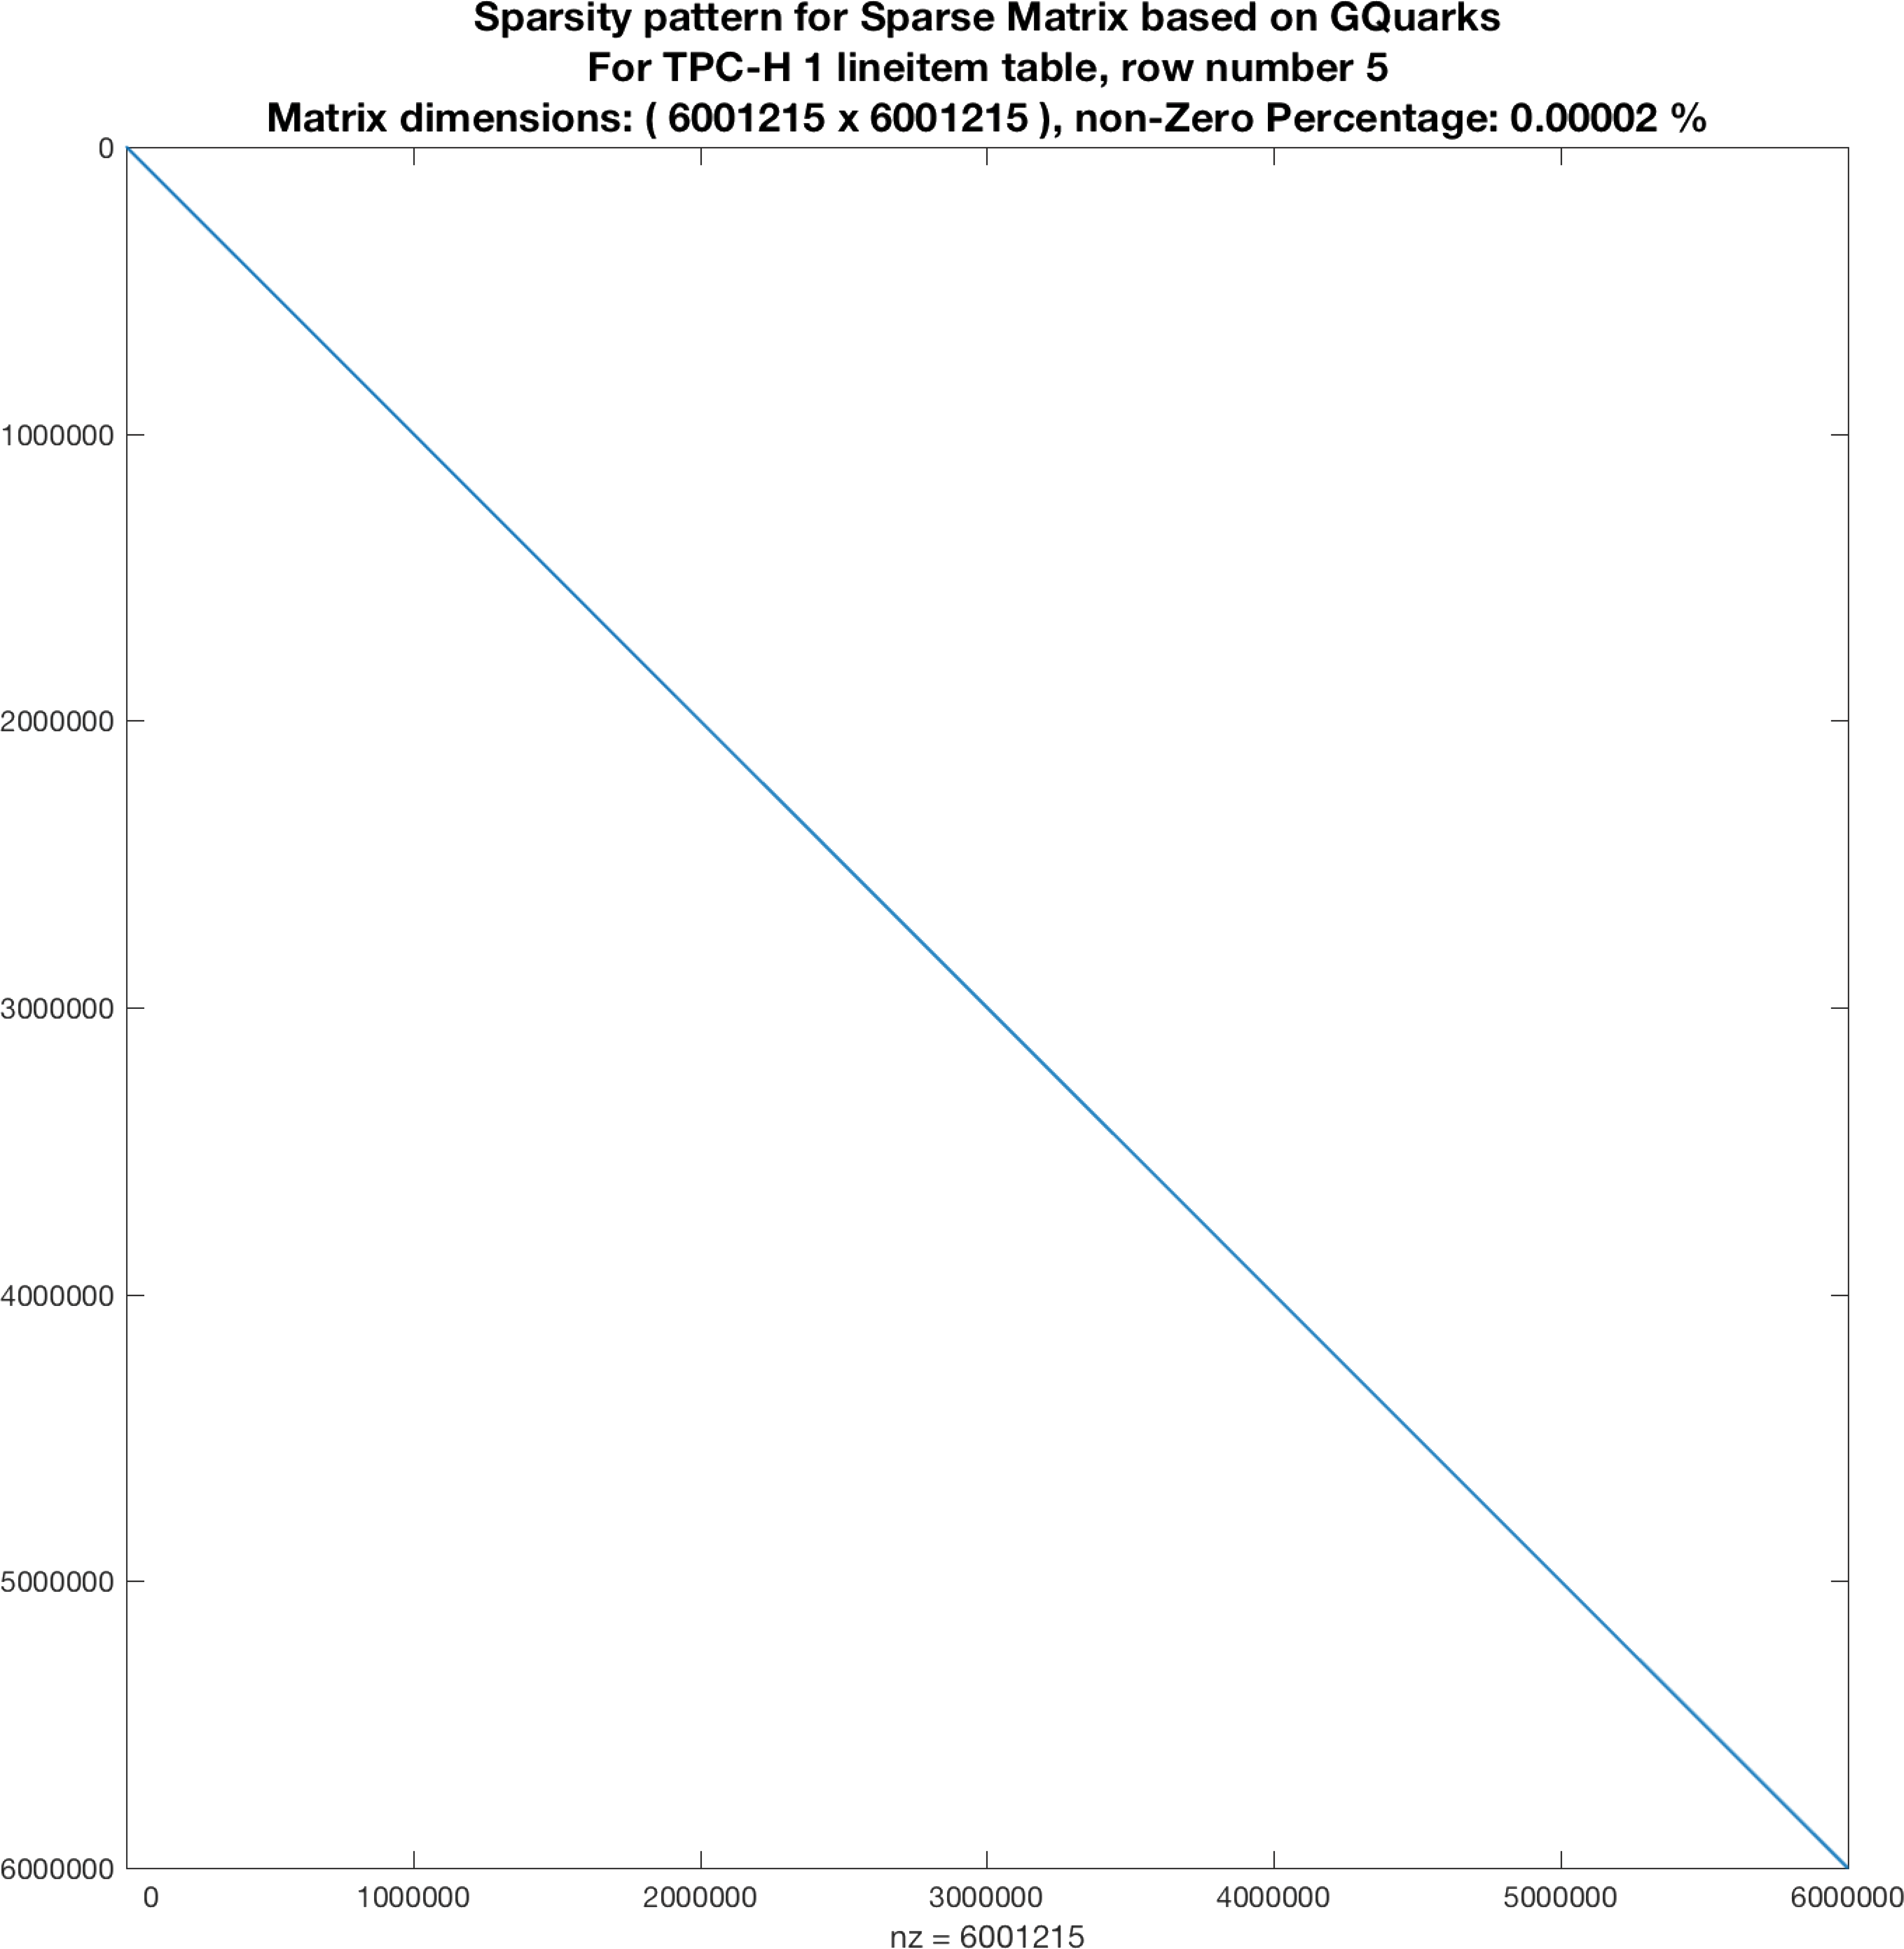
\includegraphics[width=1\columnwidth]{eps/sparsity_5.png}
\label{fig:sparse_1_5}
\end{figure}

\vspace{1.5cm}
\begin{figure}[H]
\centering
\caption{Sparsity pattern analysis for attribute return flag, from the TPC-H dataset 1GB lineitem table(column \#9).}
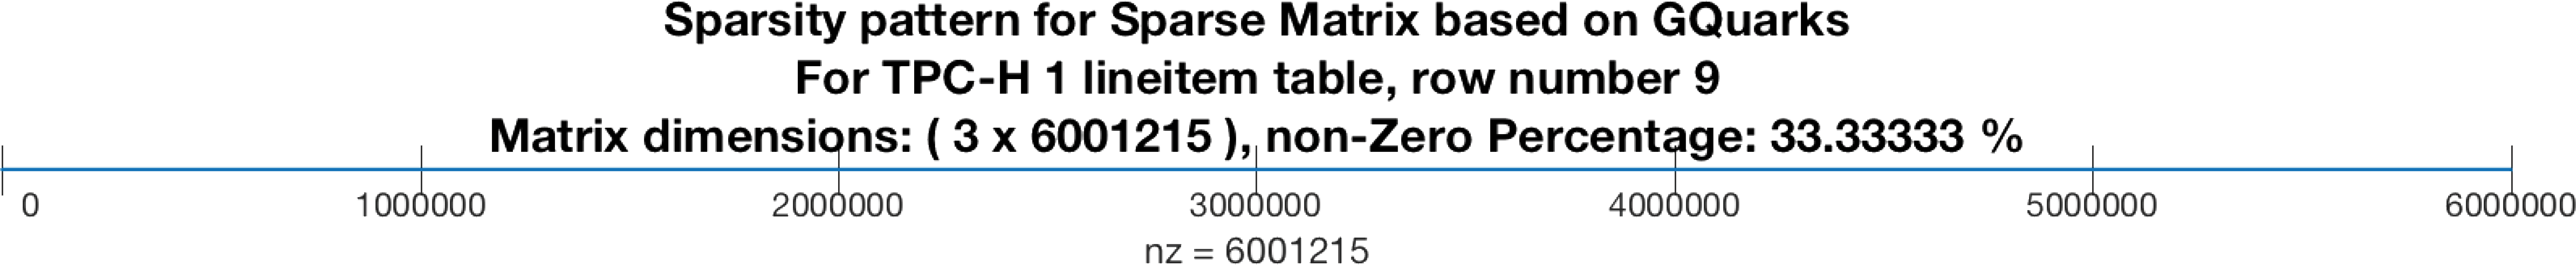
\includegraphics[width=1\columnwidth]{eps/sparsity_9.png}
\label{fig:sparse_1_9}
\end{figure}
\vspace{1.5cm}

\begin{figure}[H]
\centering
\caption{Sparsity pattern analysis for attribute line status, from the TPC-H dataset 1GB lineitem table(column \#10).}
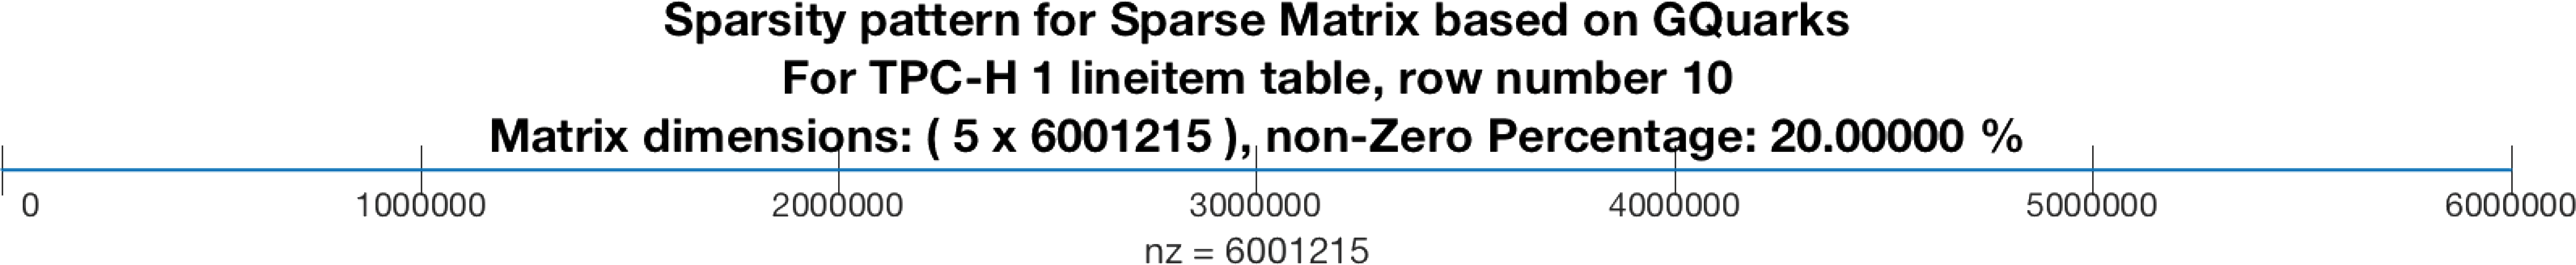
\includegraphics[width=1\columnwidth]{eps/sparsity_10.png}
\label{fig:sparse_1_10}
\end{figure}
\vspace{1.5cm}

\begin{figure}[H]
\centering
\caption{Sparsity pattern analysis for attribute shipdate, from the TPC-H dataset 1GB lineitem table(column \#11).}
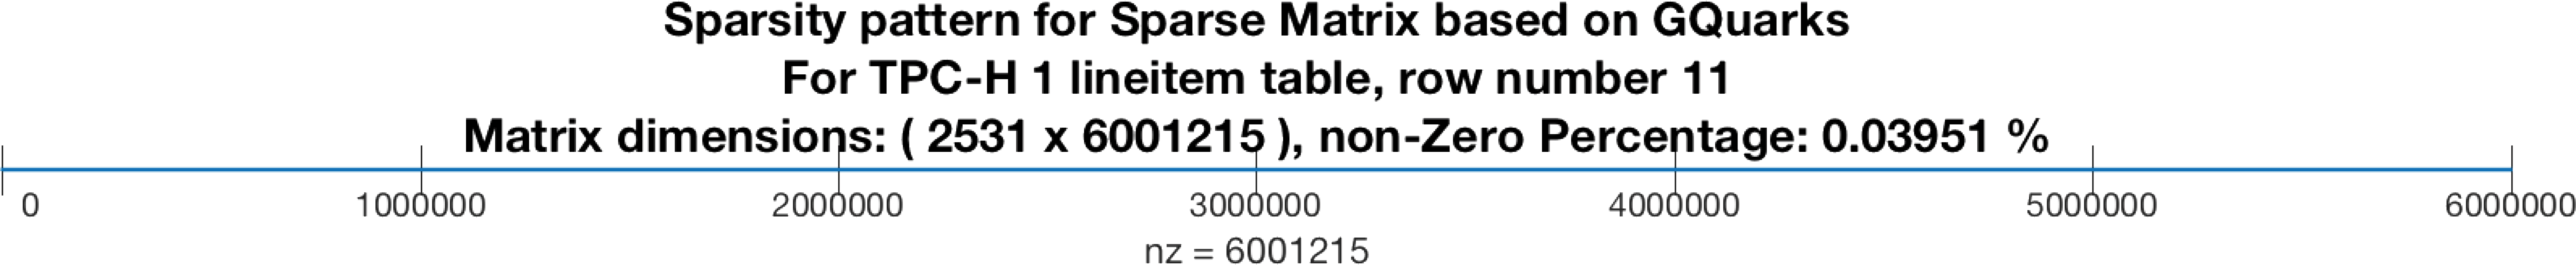
\includegraphics[width=1\columnwidth]{eps/sparsity_11.png}
\label{fig:sparse_1_11}
\end{figure}
\vspace{1.5cm}


As shown in the prior sparsity analysis, a matrix dimensions $(\ m\ \times\ n\ )$ will have, in the worst case, a non-zero number equal to n, since each column has at most one element. Therefore, to fully realise the potential of the processing units,  this memory bottleneck should be overcome.\par 
 Given the example matrix of figure \ref{fig:sparse_1_5}, the number of zero elements that would have to be stored and processed would be $(n-1)^2$. 
 
 Taking into account that for the 32GB TPC-H dataset  the number o element arises to 192,000,551, the necessary amount of memory to store only one single precision dense matrix would be  aproximately 150PB. \par 
 To explore data locality in cache memories to improve performance the design of the code should be consistent with the design of the caches. 
 The used matrices must also be compressed to take advantage of their mathematical structure. With the prior statements in mind the storage formats chosen  rely on the Compressed Sparse Column (CSC) and Compressed Sparse Row (CSR) formats \cite{silva2005sparse}. \par 
 Since each column has at most one element, the CSC format construction is thereby simplified, giving place to an sequential column pointer array, bigger in size in one element when compared to the value and row index arrays. Denote that after the LA selection operation the column pointer array no longer keeps the illustrated property. \par 
Regarding the usage of CSR format, it was chosen due to the creation of an alternative version to the LA operations that took CSC formatted matrices as input. This alternative version took CSR formatted matrices as input and relied on  Intel\textsuperscript{\textregistered} Math Kernel Library version 11.3.



\subsection{Incremental construction}
Projection matrices, as defined on section \ref{definition_matrices} are amenable to incremental construction due to the GQuarks lema, where each unique string will be associated to an unique unsigned integer. If the new data does not exist in terms of a GQuark, a new association will be created and a new unique unsigned integer will be associated to it. Regarding the consequent matrix column increase, due to register addition, no problem arises from that action.\par 
Dimension matrices, also defined on section \ref{definition_matrices}, only depend on the matrix column increase due to the direct association of the cell value, having also no problem regarding incremental construction.
Yesterday's data will still be valid and have zero migration cost with the addition of today's data.



    
 


\section{Sequential Experimentation}
\label{sequential}
\indent

Regarding the prior described lemas, we shall now assess wether if the linear algebra approach presents performance improvements when compared with the relational one. 
Before we discuss the measured performance results in the following section, we will briefly summarise characteristics of the multicore platform in our test suite, and present an overview of the performed tunings.\\

Throughout all experiments, the same platform was used. The system, referenced as compute node 652-1, has two Intel\textsuperscript{\textregistered} Xeon\textsuperscript{\textregistered} E5-2670v2 (Ivy Bridge architecture) sharing 64 GB of DDR3 RAM, 1333 MHz, accessed through 4 memory channels. Table \ref{table:characterization} fully characterises the hardware features of the test platform:

\begin{table}[H]
\centering
  \begin{tabular}{ | L{3.5cm} | R{5cm} | }
  
    \hline
    System & compute-652-1 \\ \hline \hline
        \# CPUs & 2\\ \hline
    CPU & Intel\textsuperscript{\textregistered} Xeon\textsuperscript{\textregistered} E5-2670v2\\ \hline 
    Architecture & Ivy Bridge \\ \hline 
    \# Cores per CPU & 10 \\ \hline 
    \# Threads per CPU & 20\\ \hline 
    Clock Freq. & 2.5 GHz\\ \hline \hline 
    L1 Cache & 320KB \newline 32KB per core\\ \hline 
    L2 Cache & 2560KB  \newline  256KB per core \newline\\ \hline 
    L3 Cache & 25600KB \newline shared \\ \hline \hline 
    Inst. Set Ext. & SSE4.2 \& AVX \\ \hline 
        \#Memory Channels & 4\\ \hline \hline

    Vendors Announced Peak Memory BW & 59.7 GB/s\\ \hline
    Measured\footnote{Stream Benchamrk} Peak Memory BW & 58.5GB/s\\ \hline
  \end{tabular}
     \caption{Architectural characteristics of the evaluation platform.}
     \label{table:characterization}
\end{table}

The software used for both relational and linear algebra, and the corresponding versions are stated bellow:

\begin{itemize}
\item Linear Algebra: 
    \begin{itemize}
    \item Compiler: ICC version 16.0.0 (GCC version 4.4.6 compatibility)
    \begin{itemize}
        \item no vectorization: -O3 -std=c99 -no-vec -farray-notation 
        \item vectorization: -O3 -std=c99 -farray-notation -xAVX -vec-report7
    \end{itemize}
    \item Intel\textsuperscript{\textregistered} MKL Version	11.3
    \begin{itemize}
        \item Link line: -lmkl\_intel\_lp64 -lmkl\_core -lmkl\_sequential -lpthread -lm
    \end{itemize}
        \end{itemize}

\vspace{0.35cm}
    \item Relational Algebra (PostgreSQL version 9.6+);
    \begin{itemize}
        \item Built with the following dependencies:
        \begin{itemize}
            \item GCC version 4.9.0
            \item Python 2.6.6
        \end{itemize}
           \end{itemize}
\end{itemize}

PostgreSQL was compiled specifically for the test platform, to fully take advantage of the available computing resources. 

\subsection{Tuning the relational algebra engine}
Database, application, and storage servers ship with a large number of configuration parameters like buffer cache sizes, number of I/O daemons, and parameters input to the database query optimiser. Finding good settings for these parameters is a challenging task because of the complex ways in which parameter settings can affect performance. The parameters shared\_buffers, effective\_cache\_size, and work\_mem, were adjusted accordingly, with  shared\_buffers begin set to 2GB, effective\_cache\_size being set to 64GB, and work\_mem being set to 25MB. In order to further speed up RA queries, indexes were created for all the database tables.


\subsection{Tuning sparse CSC and CSR methods to assist data level parallelism}

Efficient SSE vectorisation was achieved  in both versions of the linear algebra approach. The usage of the performant Intel Math Kernel Library (MKL) fully assisted vectorisation of the dot product between sparse matrices and sparse matrix vector, on the CSR version.\par 
The compiler was also instructed via auto vectorisation hints, and user mandated vectorisation. The non existence of vector dependencies, when verified, was also explicitly included.\par 
Alignment of data and data structures can affect performance. 
In the memory allocation alignment all data was aligned  according to cache line size. Regarding the access alignment,
for AVX, alignment to 32-byte boundaries (8 SP chunks) allowed a single reference to a cache line to move 8-SP numbers into the registers. 
The compiler was instructed to to assume that all CSC and CSR arrays are aligned on an 32-byte boundary.

\subsection{Tuning RA and LA approaches}


We conducted experiments on the simplified TPC-H  query-1, shown in listing \ref{used_query_1}, similar to the one presented in listing \ref{query_1}. 
The experiments focused a variety of datasets ranging from 1GB to 32GB. An overview of their characteristics appears in table \ref{table:dataset_info}. 

The CSC format requires a  larger  overall space for data, but it allowed us to simplify several algorithms and improve the overall perfomance.

\lstinputlisting[caption=SQL code for the simplified TPC-H query 1 used on the experimentation, label=used_query_1]{sql/used_query_1.sql} %input de um ficheiro





\end{multicols}

\noindent

\begin{table}[H]
\centering
  \footnotesize
     \caption{Overview of the produced sparse matrices used in evaluation study.}
  \begin{tabular}{ | L{0.75cm} | L{3.25cm} | L{3.25cm} | L{3.25cm} | L{3.25cm} | L{1.1cm} | L{1.1cm} | }
  
    \hline
    
  \multirow{2}{*}{Dataset} 	&	Measure Matrix Quantity			&	Projection Matrix return flag			&	Projection Matrix line status			&	Projection Matrix ship date			&	\multicolumn{2}{| L{2.4cm} |}{Overall SP Space Required}			  \\ \cline{2-7}

	&	Dimensions, Nonzeros, CSR space, CSC space			&	Dimensions, Nonzeros, CSR space, CSC space			&	Dimensions, Nonzeros, CSR space, CSC space			&	Dimensions, Nonzeros, CSR space, CSC space			&	CSR format	&	CSC format	  \\ \hline
1	& (	6001215	$\times$	6001215	) & (	3	$\times$	6001215	) & (	5	$\times$	6001215	) & (	2531	$\times$	6001215	) &		&		  \\ \cline{2-5}
	&	nnz:		6001215	&	nnz:		6001215	&	nnz:		6001215	&	nnz:		6001215	&		&		  \\ \cline{2-5}
	& CSR:	69	 MB CSC: 	69	MB & CSR:	46	 MB CSC: 	69	MB & CSR:	46	 MB CSC: 	69	MB & CSR:	46	 MB CSC: 	69	MB &	206	MB &	275	MB  \\ \hline
2	& (	11997996	$\times$	11997996	) & (	3	$\times$	11997996	) & (	5	$\times$	11997996	) & (	2531	$\times$	11997996	) &		&		  \\ \cline{2-5}
	&	nnz:		11997996	&	nnz:		11997996	&	nnz:		11997996	&	nnz:		11997996	&		&		  \\ \cline{2-5}
	& CSR:	137	 MB CSC: 	137	MB & CSR:	92	 MB CSC: 	137	MB & CSR:	92	 MB CSC: 	137	MB & CSR:	92	 MB CSC: 	137	MB &	412	MB &	549	MB  \\ \hline
4	& (	23996604	$\times$	23996604	) & (	3	$\times$	23996604	) & (	5	$\times$	23996604	) & (	2531	$\times$	23996604	) &		&		  \\ \cline{2-5}
	&	nnz:		23996604	&	nnz:		23996604	&	nnz:		23996604	&	nnz:		23996604	&		&		  \\ \cline{2-5}
	& CSR:	275	 MB CSC: 	275	MB & CSR:	183	 MB CSC: 	275	MB & CSR:	183	 MB CSC: 	275	MB & CSR:	183	 MB CSC: 	275	MB &	824	MB &	1098	MB  \\ \hline
8	& (	47989007	$\times$	47989007	) & (	3	$\times$	47989007	) & (	5	$\times$	47989007	) & (	2531	$\times$	47989007	) &		&		  \\ \cline{2-5}
	&	nnz:		47989007	&	nnz:		47989007	&	nnz:		47989007	&	nnz:		47989007	&		&		  \\ \cline{2-5}
	& CSR:	549	 MB CSC: 	549	MB & CSR:	366	 MB CSC: 	549	MB & CSR:	366	 MB CSC: 	549	MB & CSR:	366	 MB CSC: 	549	MB &	1648	MB &	2197	MB  \\ \hline
16	& (	95988640	$\times$	95988640	) & (	3	$\times$	95988640	) & (	5	$\times$	95988640	) & (	2531	$\times$	95988640	) &		&		  \\ \cline{2-5}
	&	nnz:		95988640	&	nnz:		95988640	&	nnz:		95988640	&	nnz:		95988640	&		&		  \\ \cline{2-5}
	& CSR:	1099	 MB CSC: 	1099	MB & CSR:	732	 MB CSC: 	1099	MB & CSR:	732	 MB CSC: 	1099	MB & CSR:	732	 MB CSC: 	1099	MB &	3296	MB &	4394	MB  \\ \hline
32	& (	192000551	$\times$	192000551	) & (	3	$\times$	192000551	) & (	5	$\times$	192000551	) & (	2531	$\times$	192000551	) &		&		  \\ \cline{2-5}
	&	nnz:		192000551	&	nnz:		192000551	&	nnz:		192000551	&	nnz:		192000551	&		&		  \\ \cline{2-5}
	& CSR:	2197	 MB CSC: 	2197	MB & CSR:	1465	 MB CSC: 	2197	MB & CSR:	1465	 MB CSC: 	2197	MB & CSR:	1465	 MB CSC: 	2197	MB &	6592	MB &	8789	MB  \\ \hline
  \end{tabular}
     \label{table:dataset_info}
\end{table}
\vspace{2cm}

\begin{multicols}{2}


\subsection{Experimental results analysis}

Figure \ref{fig:time_la_vs_ra} plots the measured execution for a range of datasets, and both linear and relational algebra approaches.

Denote that the presented values were selected through the K-Best technique, with K=3, from 50 samples. 

For the linear algebra approach we present the best solution from CSR and CSC format. The presented linear algebra solution in figure \ref{fig:time_la_vs_ra} is the one using CSR and format and  Intel MKL version 11.3. \par
The experiment presented in the current section focus on the best possible sequential solutions for both relational and linear algebra versions. The parallel PostgreSQL line was only introduced to elucidate the parallel  goal to achieve in the LA versions discussed in later sections of this report, and discuss future potential improvements of our linear algebra system. 

As shown, the coding effort to tune sparse CSR methods to assist data level parallelism revealed itself fruitful. However, a further analysis should be produced in order to fully potentiate vectorisation opportunities and optimisations.\par 

\begin{figure}[H]
\centering
\caption{Execution time for the  simplified query-1 from TPC-H benchmark, for different scale factors (dataset sizes from 1GB to 32GB).}
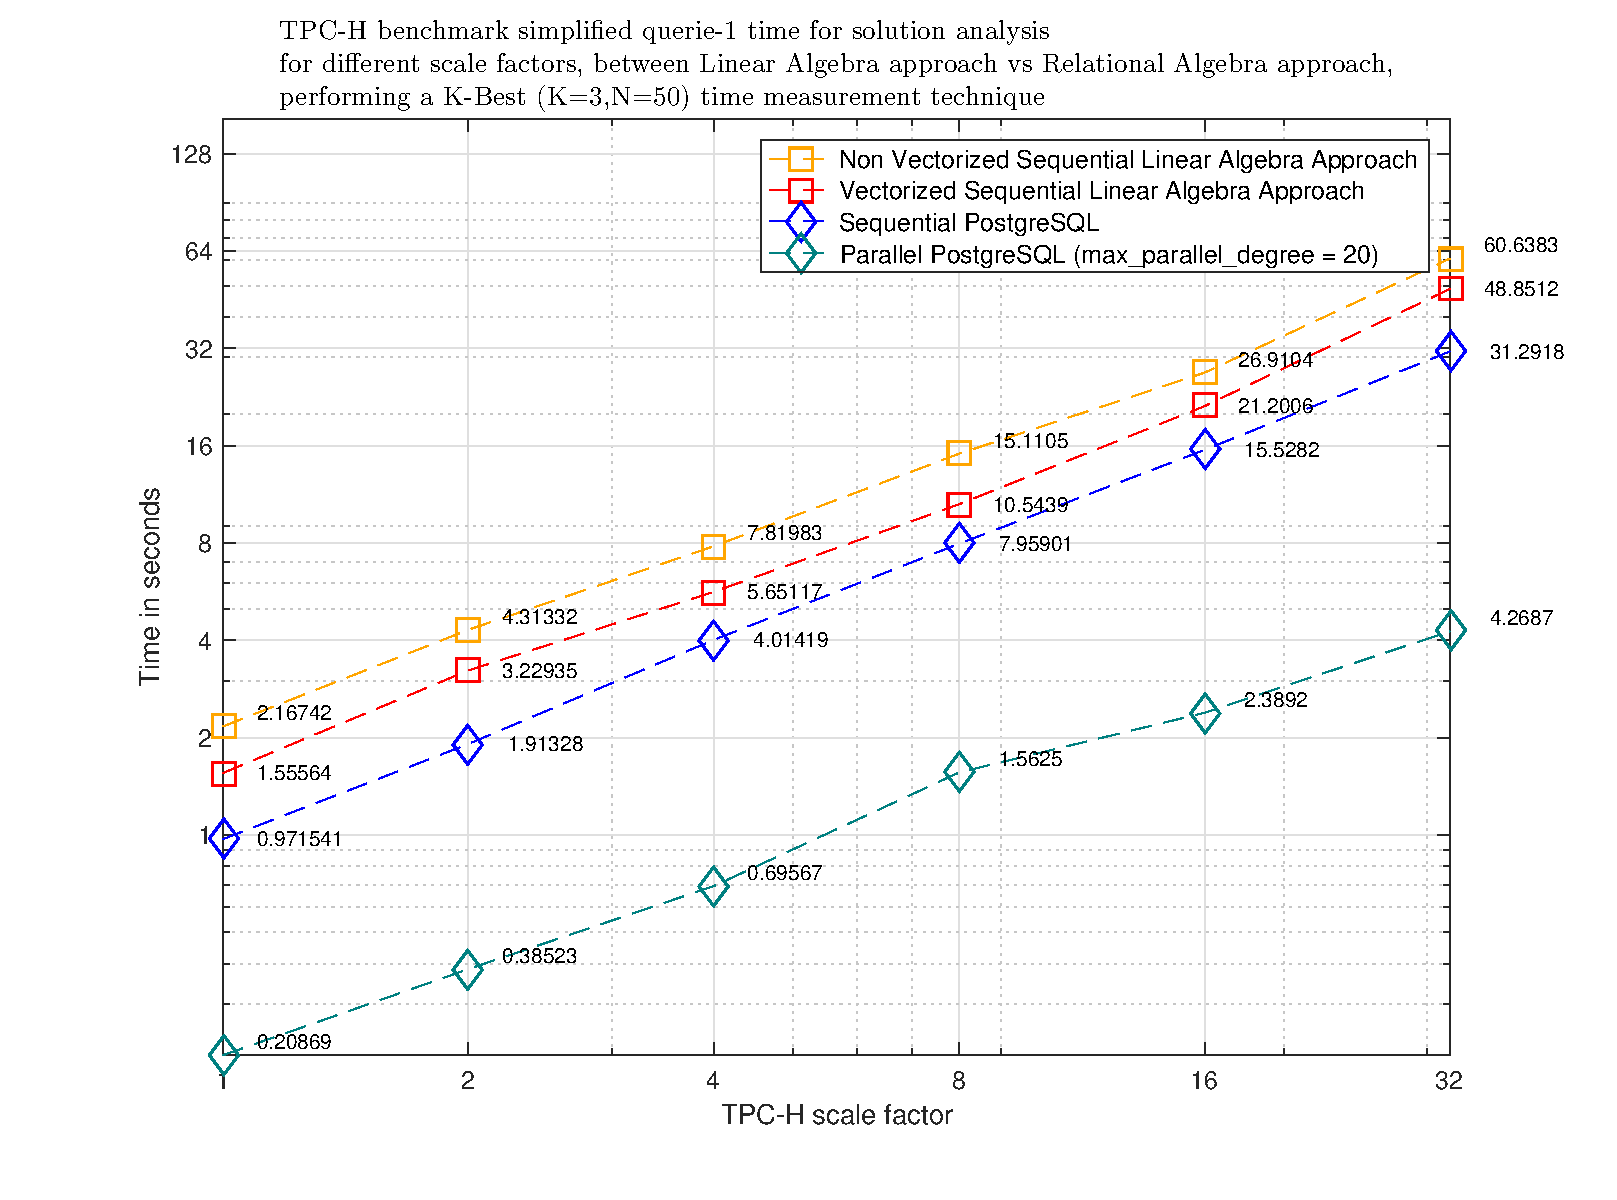
\includegraphics[width=1\columnwidth]{eps/TIME_LA_vs_RA_1st.eps}
\label{fig:time_la_vs_ra}
\end{figure}





\newpage
\section{Parallelisation}
\label{parallel}
\indent
\par 

\subsection{Sequential Profiling}
Prior to parallelisation every step of the linear algebra expression was profiled to identify potencial hotspots. Since the best parallel linear algebra version turned out to be the CSC version, special attention is added to it when compared to the CSR version. \par 
Table \ref{table:profile_seq} displays the profiler results for  the CSC version with the largest TPC-H dataset in test - 32GB, namely the percentage of overall time for each operation present in expression \ref{eq:tpch_1}.

\begin{table}[H]
\centering
\footnotesize
  \begin{tabular}{ | L{1cm} | L{1.25cm} |  L{1.2cm} |  L{1.3cm} |  L{1.6cm} | L{1cm} |  }
    \hline
    LA Version	&	Projection	&	Selection	&	Projection . Selection	&	(Projection .Selection). Quantity	&	Bang	\\ \hline
Seq. CSC	&	23.93\%	&	43.38\%	&	10.89\%	&	18.12\%	&	3.68\%	\\ \hline
  \end{tabular}
     \caption{Profiling results for the sequential CSC linear algebra version, for TPC-H 32GB dataset, for the evaluation platform.}
     \label{table:profile_seq}
\end{table}

As shown in table \ref{table:profile_seq}, the most time consuming operations are the selection and the projection (Khratri-Rao operation). Further efforts to reduce the selection overhead are discussed in subsection \ref{optimization_selection}. \par 

\subsection{Parallel Experimental Results and Analysis}

To parallelise both linear algebra versions, in a multicore system, we opted by OpenMP version 4.0.
Using the CSC format in the linear algebra version the algorithms offer good parallelisation opportunities, since each column has at most one element. 

To parallelise with the CSR format the algorithms are more challenging. \par 

Figure \ref{fig:time_la_vs_ra_parallel} presents the measured execution times for a wide range of datasets, and for both linear and relational algebra approaches. The presented values were selected through the K-Best technique, with K=3 from 50 samples. For the linear algebra approach we present the the best execution times for the best CSR and CSC formats, namely the CSC format version.\par

As shown, the parallel linear algebra approach is faster than the parallel relational algebra, although larger TPC-H datasets reduce the gain from the linear algebra approach. Further algorithm optimisation will be discussed in  subsection \ref{optimization_selection}.\par 

\begin{figure}[H]
\centering
\caption{TPC-H benchmark simplified query-1 time for solution analysis for different scale factors, between parallel linear and relational algebra approaches.}
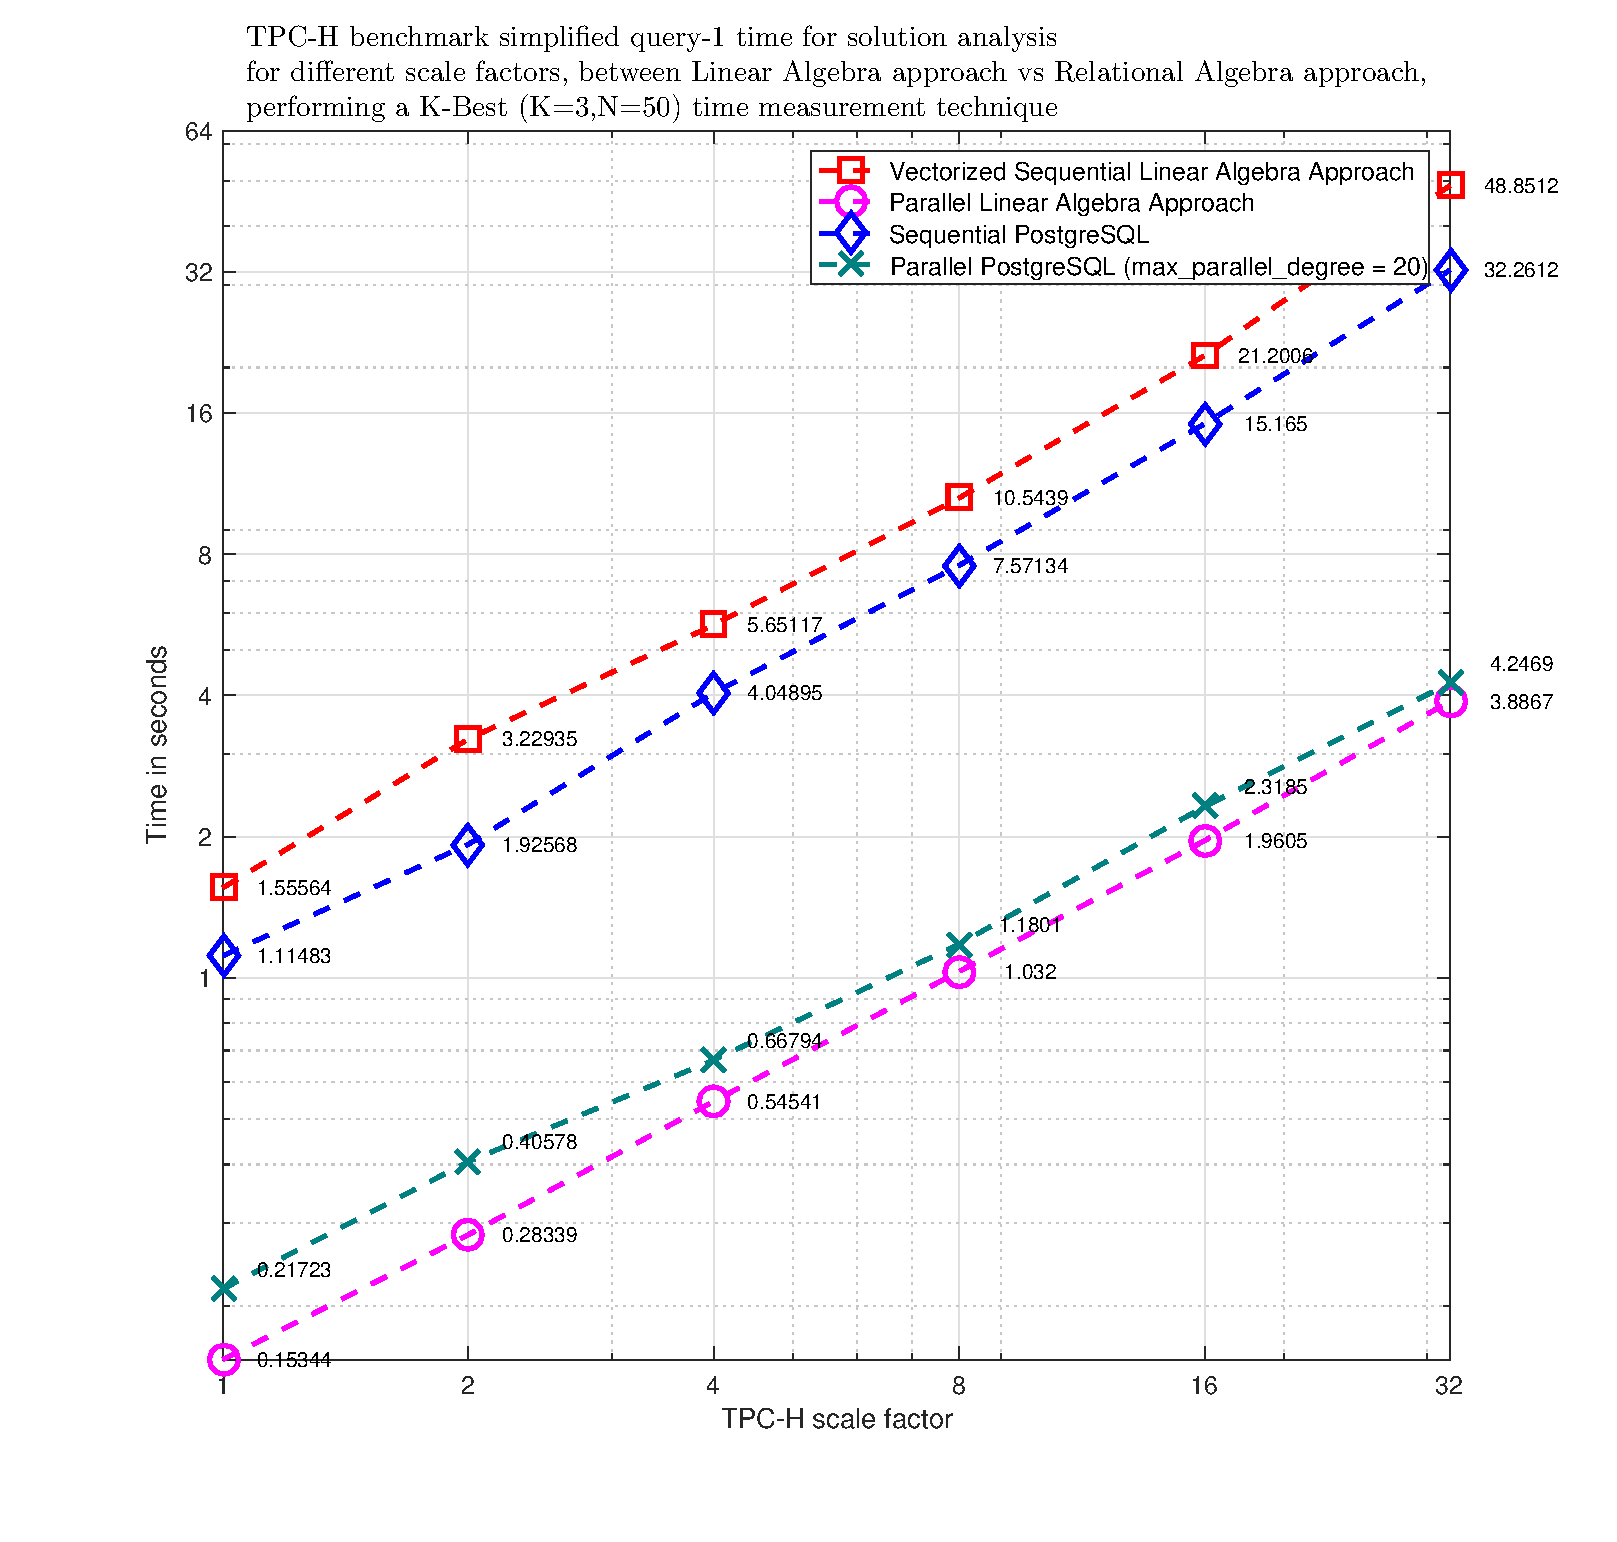
\includegraphics[width=1\columnwidth]{eps/TIME_LA_vs_RA_parallel.eps}
\label{fig:time_la_vs_ra_parallel}
\end{figure}

\subsection{Further Selection Algorithm Optimisation}
\label{optimization_selection}

Further profiling was made to better identify the potential bottlenecks. Table \ref{table:profile_par} compares both sequential and parallel linear algebra versions. The projection operation has decreased the percentage of overall time to complete the operation. However, the selection operation has increased its overall time percentage  to almost half the overall value. \par 


\begin{table}[H]
\centering
\footnotesize
  \begin{tabular}{ | L{1cm} | L{1.25cm} |  L{1.2cm} |  L{1.3cm} |  L{1.6cm} | L{1cm} |  }
    \hline
    LA Version	&	Projection	&	Selection	&	Projection . Selection	&	(Projection .Selection). Quantity	&	Bang	\\ \hline
Seq. CSC	&	23.93\%	&	43.38\%	&	10.89\%	&	18.12\%	&	3.68\%	\\ \hline
Par. CSC	&	13.62\%	&	46.83\%	&	11.49\%	&	16.74\%	&	3.51\%	\\ \hline

  \end{tabular}
     \caption{Profiling results for the parallel CSC linear algebra version, for TPC-H 32GB dataset, for the evaluation platform.}
     \label{table:profile_par}
\end{table}

After a careful examination of a portion the C source code for the CSC version selection, in listing \ref{selection_code_old}, further algorithm optimisations can be made. 

\newpage
\lstinputlisting[caption=Portion of the C source code for the CSC linear algebra version selection algorithm, label=selection_code_old]{src/selection_old.c} 

Taking as example the TPC-H 32GB dataset, and the shipdate matrix, with dimension $(\ m\ \times\ n\ ), namely $(\ 2,531\ $\times\ 192,000,551\ )$, to compute the selection result, in the worst case scenario, it is necessary to realize $(n * 2) = 384,001,102 $ string comparisons. However, by analysing table \ref{table:dataset_info}, from the 384,001,102 string comparisons only 2,531 distinct strings will be tested.\par 
 Listing \ref{selection_code_new} avoids repetitive string comparisons  by adding an additional auxiliar array (of size n), resulting in a worst case scenario of  $(m * 2) = 5,062 $ string comparisons and $n = 192,000,551 $ integer comparisons.\par
 This solution resolves two distinct problems:  the excessive overhead of accessing a large amount and repetitive string comparisons, and the improvement of this solution with bigger datasets. 
 The additional overhead of producing an auxiliar array gets diminished with the increase of the dataset  and consequently the required comparisons.  The larger the dataset, the better. 

\lstinputlisting[caption=Portion of the C source code for the CSC linear algebra version selection algorithm, label=selection_code_new]{src/selection_new.c} 

Table \ref{table:profile_par_new} compares three parallel linear algebra versions: the sequential, the parallel, and an optimised parallel version. The selection operation largely diminished its percentage overall time making it possible for the overall time to be averagely distributed among operations. \par 

\begin{table}[H]
\centering
\footnotesize
  \begin{tabular}{ | L{1cm} | L{1.25cm} |  L{1.2cm} |  L{1.3cm} |  L{1.6cm} | L{1cm} |  }
    \hline
    LA Version	&	Projection	&	Selection	&	Projection . Selection	&	(Projection .Selection). Quantity	&	Bang	\\ \hline
Seq. CSC	&	23.93\%	&	43.38\%	&	10.89\%	&	18.12\%	&	3.68\%	\\ \hline
Par. CSC	&	13.62\%	&	46.83\%	&	11.49\%	&	16.74\%	&	3.51\%	\\ \hline
Optimized Par. CSC	&	10.47\%	&	20.10\%	&	25.86\%	&	34.60\%	&	8.98\%	\\ \hline
  \end{tabular}
     \caption{Profiling results for the selection algorithm optimised parallel CSC linear algebra version, for TPC-H 32GB dataset, for the evaluation platform.}
     \label{table:profile_par_new}
\end{table}

\subsection{Final Parallel Experimental Results}

Figure \ref{fig:time_la_vs_ra_parallel_v2} presents the measured execution times for a wide range of datasets, and both linear and relational algebra approaches.   The presented values were selected through the K-Best technique, with K=3 from 50 samples. 
For the linear algebra approach we present the the best solution with the CSC format, in the optimised parallel version.\par
As shown, the parallel linear algebra solution in both versions is faster than the parallel relational algebra, and the speedup was stable for whole range of  TPC-H datasets.\par 
Figure \ref{fig:speedup_la_vs_ra_parallel} plots the obtained speedups between sequential LA and parallel LA versions, and between the parallel LA and RA versions.

\begin{figure}[H]
\centering
\caption{TPC-H benchmark simplified query-1 time for solution analysis for different scale factors, between parallel linear and relational algebra approaches, in which linear algebra approach states the selection algorithm optimisation.}
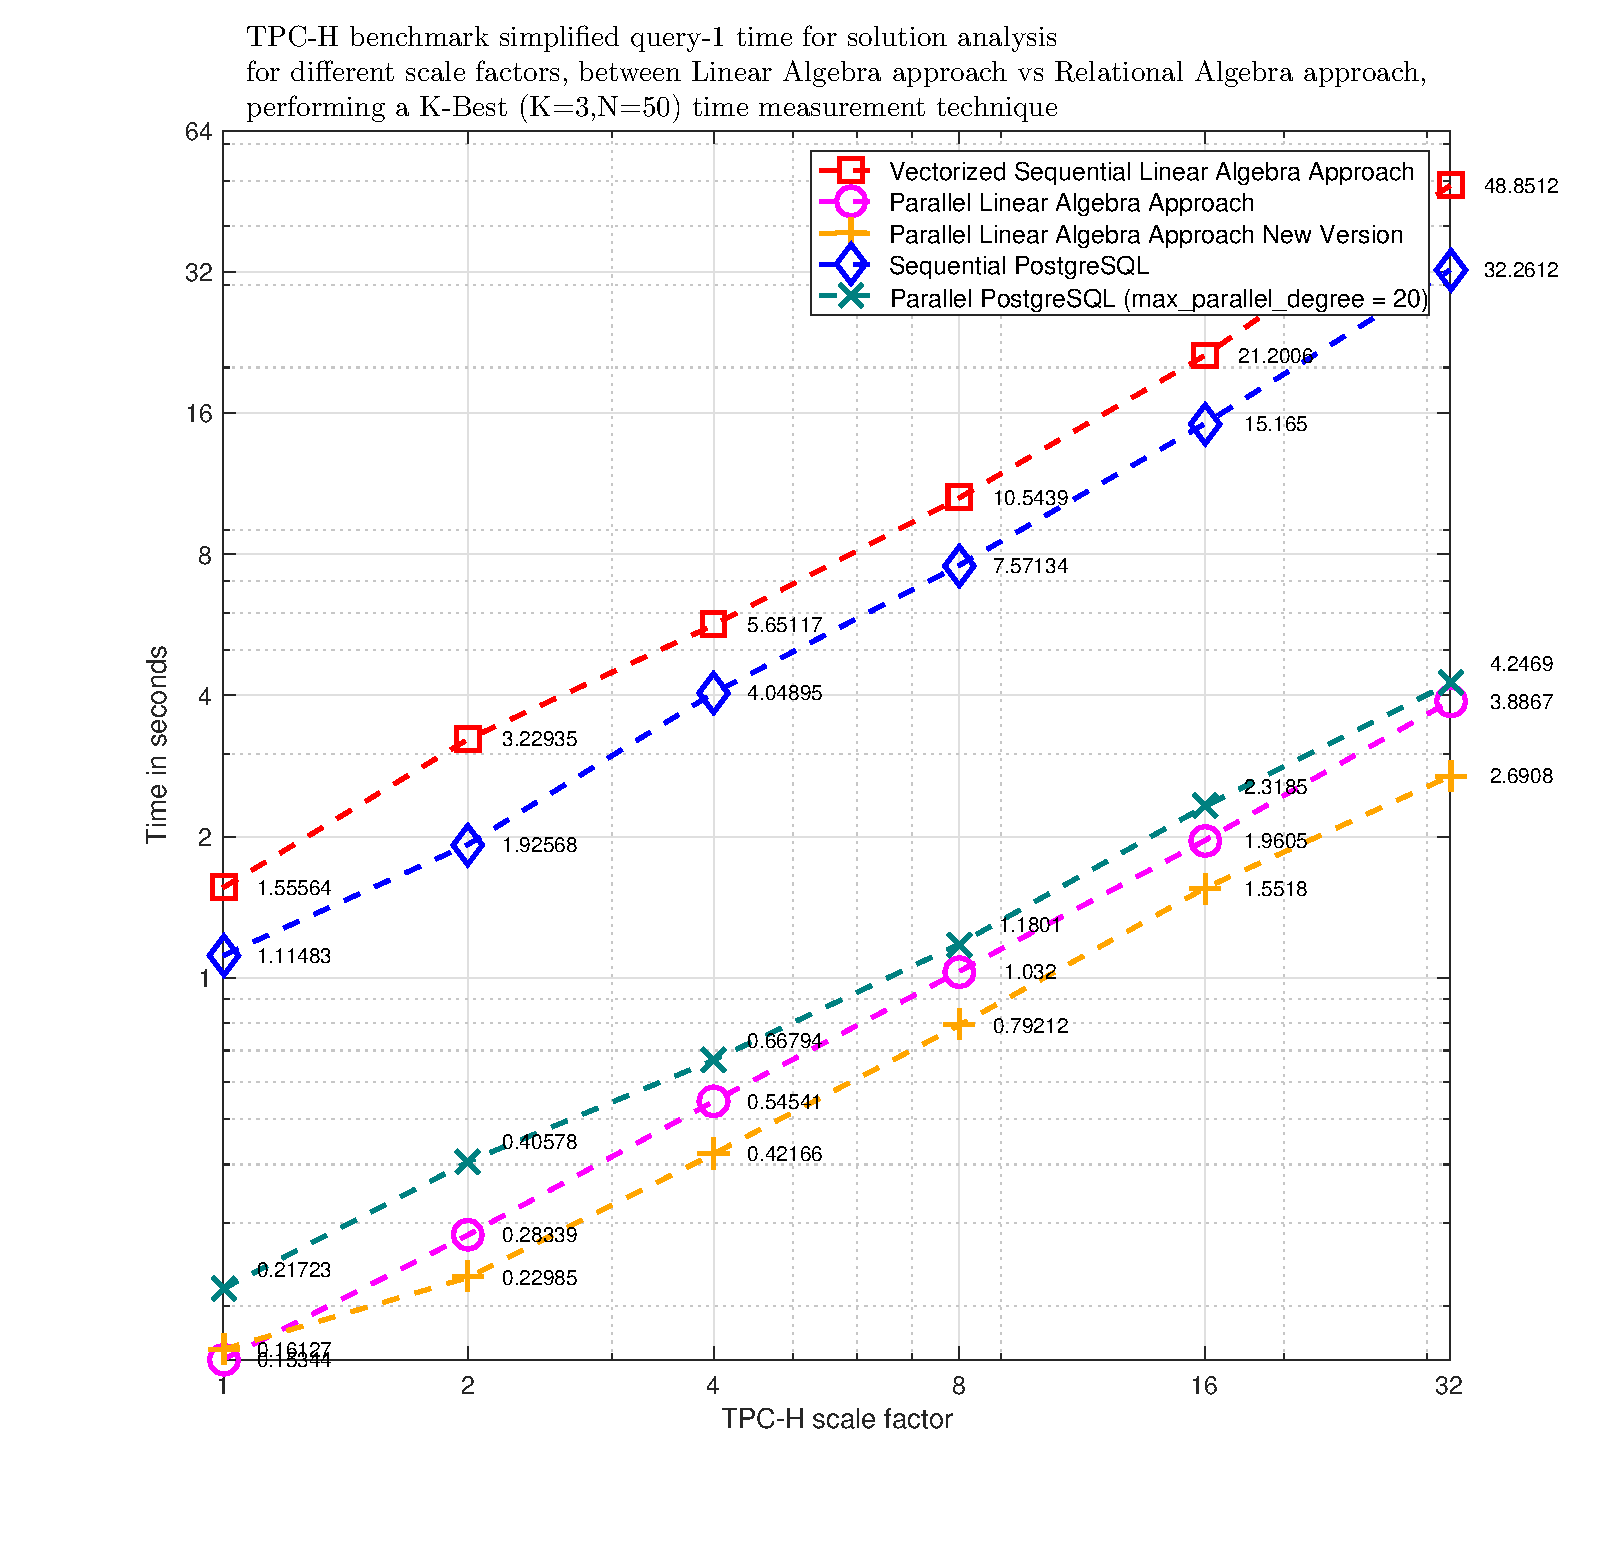
\includegraphics[width=0.95\columnwidth]{eps/TIME_LA_vs_RA_parallel_v2.eps}
\label{fig:time_la_vs_ra_parallel_v2}
\end{figure}


\begin{figure}[H]
\centering
\caption{TPC-H benchmark simplified query-1 speedup analysis for different scale factors, between sequential linear algebra vs parallel linear algebra and parallel linear algebra vs parallel relational algebra.}
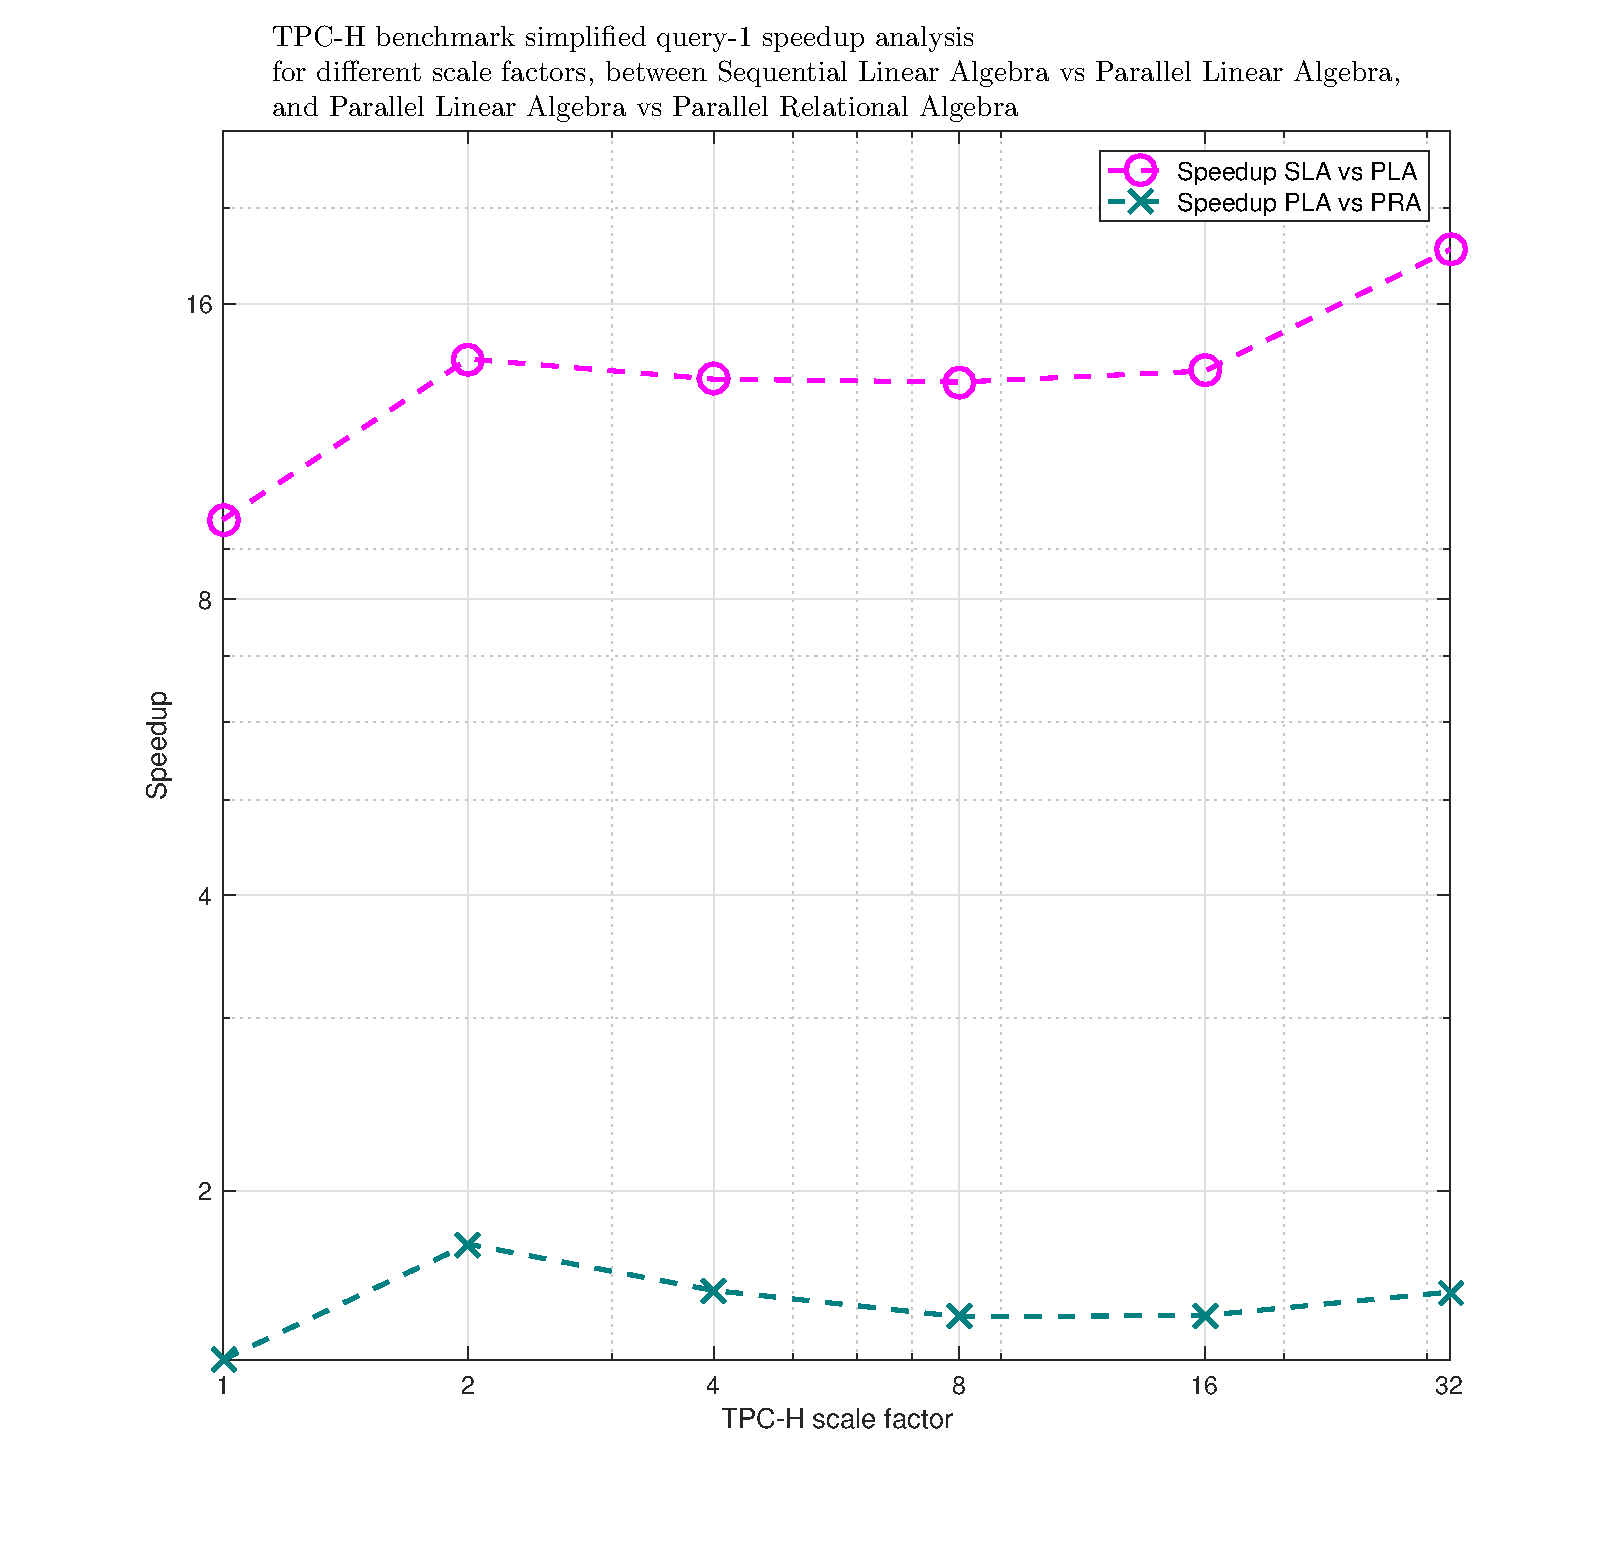
\includegraphics[width=0.95\columnwidth]{eps/speedup.eps}
\label{fig:speedup_la_vs_ra_parallel}
\end{figure}




\section{Conclusion}
\indent
\label{conclusion}

We have designed, implemented and evaluated an efficient and parallel LA framework to provide fast responses to OLAP queries in very large databases. We started by developing a typed linear algebra solution to respond to OLAP TPC-H query 1, with faster response times than a Open Source relational algebra competitor, PostgresSQL. 

A challenge in this project was to understand the linear algebra theory prior defined\cite{macedo2015linear} \cite{Po15}, to fully represent relational algebra in terms of linear algebra operators. This process was longstanding and it was only managed to do it with help of our advisors. Efforts were made to correctly introduce the key ideias prior presented\cite{macedo2015linear}, and resolving potential difficulties that the previous implementations faced. \par


%N�O SEI O QUE O PROFESSOR QUER COM A LINHA AO LADO DESTE PARAGRAFO
In spite the already 18x speedup regarding sequential linear algebra version and the 2x speedup regarding the parallel relational algebra engine, a lot of work can be done to further improve the algorithm, and fully analyse TPC-H queries results, as stated on section \ref{future_work}, leaving several potential exploratory paths.

 





\section{Future Work}
\label{future_work}
\indent


The biggest problem of the linear algebra implementation can be the intermediate matrices, if a column has no nonzero element, they are not optimal for further parallelisations. This is the unique speedup 

limitation

regarding the relational algebra approach. If that limitation is overcome the speedups would climb to more significant values when compared to the relational algebra version. \par 
It is also clear that the keys for selection significantly interfere with both linear and relational algebra algorithms. In the LA specific case, a selection operation that returns a low number of nonzero elements might compromise the attainable speedup through parallelisation, since there might not be enough data to keep the computational units busy. \par 

There is still room to greatly improve the parallelisation of this algorithm. For example,  a gather/scatter analysis for distributed memory parallelism might result in larger attainable speedup. However, efforts need to me made to detect possible latency or bandwidth issues. \par 
Another approach is to duplicate data in a shared memory environment . For the CSC format, regarding the three arrays, every thread would have the total CSC column pointer array and a portion of CSC values and CSC row indexes arrays. The computation of both splitted arrays would be thread independent and there would only be necessary to reduce the CSC column pointer. \par 

To improve data locality the Block Compressed Sparse Row (BSR) Format could be used. However, it would largely increase the algorithm complexity for the defined methods. That improvement should only be used in the CSR linear algebra defined version.\par 

Future work also includes extending the scope of both offline and run-time optimisations. These include:
\begin{itemize} 
\item to fully translate the remaining TPC-H queries and benchmark both linear and relational algebra approaches;
\item to investigate reordering methods to reduce total query compute time;
\item to exploit index compression, further cache-blocking and TLB blocking to reduce memory traffic and to further improve locality;
\item to implement other matrix partitioning schemes;
\item to improve load balance when there are different data structures for each generated matrix;
\item to reduce data structure conversion costs at run-time, for the CSR linear algebra version;
\item to determine the most efficient number of cores for parallelism.
\end{itemize}

The usage of CUDA and MIC systems should also be explored as an heterogenous system solution. Since the algorithms require huge portions of simple computation, and it is already parallelised via OpenMP, porting the application to be Xeon Phi compatible should not present great challenges.\par 


 


\section{Acknowledgements}
\indent



We would like to thank our advisors for all the help they gave us and for always being available for all the questions
we had. 
We would also like to thank Rog\'erio Pontes for all the
help he gave us in understanding how the linear algebra theory would fit in OLAP, and all the time he spent helping us improve the parallel algorithms.

 
%---------------------------------------------------------------------------------------
%	REFERENCE LIST
%--------------------------------------------------------------------------------------

\bibliography{biblio}

\bibliographystyle{plain}

%---------------------------------------------------------------------------------------
\end{multicols}
\end{document}



